\documentclass[aspectratio=169]{beamer}
\usepackage{animate}

% Show notes
\usepackage{pgfpages}
%\setbeameroption{show notes on second screen}

\usepackage[utf8]{inputenc}

\setbeamertemplate{note page}
{%
  % Header box
  \insertvrule{.27\paperheight}{white!90!black}
  \vskip-0.286\paperheight
  \begin{minipage}{0.4\textwidth}
    \insertslideintonotes{0.25}%
  \end{minipage}
  \begin{minipage}{0.55\textwidth}
    {\textbf \insertshortframetitle}
  \end{minipage}

  % Title
  \begin{minipage}{0.88\paperwidth}
  \insertnote
  \end{minipage}
}

\newcommand{\timenote}[3]{
    \note{
        \vskip-0.1\paperheight
        \hspace{4.44cm}Time: #1 -- #2 min
        \vskip0.086\paperheight
        {\scriptsize #3}}
}

\usepackage{mathtools}


\usepackage[]{algorithm2e}
\usepackage{bm}
\renewcommand{\vec}[1]{%
  \ifcat\noexpand#1\relax % check if the argument is a control sequence
    \bm{#1} % probably Greek
  \else
    \mathbf{#1} % single character
  \fi
}
\usepackage{amssymb}
\usepackage{amstext}
\usepackage{amsmath}
\usepackage{amsthm}
\usepackage{changepage}
\usepackage{mathrsfs}  % Used for mathscr 'L'
\usepackage{gensymb}  % degree sign
\usepackage{bm}
\usepackage{bbm}
\renewcommand{\epsilon}{\varepsilon}
\usepackage{cancel}
%\usepackage{breqn}
%\usepackage{enumitem}
\usepackage{booktabs}
%\usepackage[table]{xcolor}
\usepackage{multirow}

%\usepackage{empheq}
%\usepackage[most]{tcolorbox}
%\newtcbox{\mymath}[1][]{%
%    nobeforeafter, math upper, tcbox raise base,
%    enhanced, colframe=blue!30!black,
%    colback=blue!30, boxrule=1pt,
%    #1}
%\tcbset{
%    enhanced,
%    breakable,
%    attach boxed title to top center,
%    top=1mm,
%    coltitle=black,
%    beforeafter skip=\baselineskip,
%}

\newcommand{\etal}{\emph{et~al.}}

% Graphics
\graphicspath{{../images/}{../matlab/}{../../camera_ready/images/}}
\DeclareGraphicsExtensions{.pdf,.jpeg,.png,.eps}

\newcommand{\FULLSCREEN}{0.65\textwidth}

% vast and Vast brackets (larger than Huge)
\makeatletter
\newcommand{\HUGE}{\bBigg@{3}}
\newcommand{\vast}{\bBigg@{4}}
\newcommand{\Vast}{\bBigg@{5}}
\makeatother

\usepackage[export]{adjustbox}[2011/08/13]


\newcommand{\cammat}[2]{\left[#1\;|\;#2\right]}
\newcommand{\R}{\ensuremath{\mathbbm{R}}}
\newcommand{\K}{\ensuremath{\mathbbm{K}}}
\newcommand{\C}{\ensuremath{\mathbbm{C}}}
\renewcommand{\P}{\ensuremath{\mathbbm{P}}}
\renewcommand{\phi}{\varphi}
\DeclareMathOperator*{\argmax}{arg\,max}
\DeclareMathOperator*{\argmin}{arg\,min}
\DeclareMathOperator{\nulldim}{nulldim}
\DeclareMathOperator{\adj}{adj}
\newcommand{\mat}[1]{\bm{#1}}
\newcommand{\nullspace}[1]{\mathcal{N}{#1}}
\newcommand{\lr}{\ensuremath{\mathrm{\quad\Leftrightarrow\quad}}}
\newcommand{\A}{\ensuremath{\mathcal{A}}}
\newcommand{\N}{\ensuremath{\mathcal{N}}}
\newcommand{\reg}{\ensuremath{\mathcal{R}}}
\newcommand{\Real}{\ensuremath{\mathbbm{R}}}
\newcommand{\Z}{\ensuremath{\mathbbm{Z}}}
\newcommand{\Tp}{T}
\newcommand{\norm}[1]{\|#1\|}
\newcommand{\frobnorm}[1]{\norm{#1}_F}
\newcommand{\fr}[2]{\frac{#1}{#2}}
\newcommand{\pf}[2]{\frac{\partial #1}{\partial #2}}
\DeclareMathOperator{\tr}{tr}
\DeclareMathOperator{\diag}{diag}
\DeclareMathOperator{\atan}{atan2}
\DeclareMathOperator{\rank}{rank}
\DeclareMathOperator{\vectorize}{vec}

\newcommand{\T}{T}
\usepackage{setspace}
%\usepackage{xcolor}
\usepackage{tikz}
\usetikzlibrary{tikzmark}
\usepackage{pgfplots}

%\usepackage{caption}
\usepackage{subcaption}

\def\thicknesslineplot{thick}
\def\thicknesshack{0.085cm}
\def\mythickness{ultra thick}
\def\thicknesslineplotTwo{thick}
\def\mythicknesssmall{thick}
\def\thicknesslineplotThree{very thick}
\def\boxplotheight{8.5cm}
\def\boxplotwidth{7.5cm}
\def\boxplotheightreal{3.5cm}

\definecolor{gtcolor}{rgb}{0,0,0}
\definecolor{ourcolor}{rgb}{0,0.4,0.6}
\definecolor{fitzgibboncolor}{rgb}{0,0.7,0.7}
\definecolor{dingcolor}{rgb}{1,0.2,0.3}
\definecolor{kukelovacolor}{rgb}{0,0.6,0}
\definecolor{bougnouxcolor}{rgb}{0,0.7,0.7}
\definecolor{valtonenoernhagcolor}{rgb}{0.7,0,0.7}
\definecolor{inliercolor}{rgb}{0.2,1,0.1}
\definecolor{outliercolor}{rgb}{1,0,0}
\definecolor{smallcolor1}{rgb}{0.,0,0}
\definecolor{smallcolor2}{rgb}{0,0,0}
\definecolor{hiddencolor}{rgb}{0.1,0.9,0.1}
\definecolor{elimcolor}{rgb}{0.6,0.1,0.6}

\makeatletter
\DeclareRobustCommand\eg{\emph{e.g}\@ifnextchar.{}{.\@}}
\DeclareRobustCommand\etal{\emph{et~al}\@ifnextchar.{}{.\@}}
\DeclareRobustCommand\ie{\emph{i.e}\@ifnextchar.{}{.\@}}
\DeclareRobustCommand\cf{\emph{cf}\@ifnextchar.{}{.\@}}
\DeclareRobustCommand\NB{\emph{N.B}\@ifnextchar.{}{.\@}}
\DeclareRobustCommand\wrt{w.r.t\@ifnextchar.{}{.\@}}
\makeatother

\newcommand{\CE}{\ensuremath{\mat{C}_\mathcal{E}}}
\newcommand{\CR}{\ensuremath{\mat{C}_\mathcal{R}}}
\newcommand{\CB}{\ensuremath{\mat{C}_\mathcal{B}}}
\newcommand{\CEk}[1]{\ensuremath{\mat{C}_{\mathcal{E}_{#1}}}}
\newcommand{\CRk}[1]{\ensuremath{\mat{C}_{\mathcal{R}_{#1}}}}
\newcommand{\CBk}[1]{\ensuremath{\mat{C}_{\mathcal{B}_{#1}}}}
\newcommand{\XE}{\ensuremath{\mat{X}_\mathcal{E}}}
\newcommand{\XR}{\ensuremath{\mat{X}_\mathcal{R}}}
\newcommand{\XB}{\ensuremath{\mat{X}_\mathcal{B}}}

\newcommand{\sing}[1]{\vec{\sigma}{#1}}
\usepackage{standalone}
\pgfplotsset{
    table/search path={../../graphs},
}

\makeatletter
\@namedef{ver@everyshi.sty}{} %Prevents some error caused by tikz, has to be agter xcolor
\makeatother
\usepackage{tikz}  % Used for problem geometry picture
\usepackage{pgfplots}
\usepackage{tikzpagenodes}
\usetikzlibrary{positioning}
\usetikzlibrary{arrows,shapes,shapes.symbols}
\usetikzlibrary{arrows.meta}
\usetikzlibrary{matrix, fit}
\tikzset{%
  thick arrow/.style={
     -{Triangle[angle=90:2pt 1.5]},
     line width=4mm,
     draw=gray,
     draw opacity=0.7,
  },
}
\tikzset{
node distance = 9em and 4em,
sloped,
   box/.style = {%
    shape=rectangle,
    rounded corners,
    draw=blue!40,
    fill=blue!15,
    align=center,
    font=\fontsize{12}{12}\selectfont},
 arrow/.style = {%
    draw=blue!30,
    line width=2mm,% <-- select desired width
    -{Triangle[length=3mm]},
    shorten >=1mm, shorten <=1mm,
    font=\fontsize{8}{8}\selectfont},
    }
\pgfplotsset{compat=1.15}
\usetikzlibrary{shapes.misc, positioning}
\usetikzlibrary{arrows}
\usetikzlibrary{calc}

\pgfdeclarelayer{foreground}  % Used for correct opacity
\pgfdeclarelayer{background}  % Used for correct opacity
\pgfsetlayers{background,main,foreground}

\DeclareGraphicsRule{.tif}{png}{.png}{`convert #1 `dirname #1`/`basename #1 .tif`.png}

\usepackage{environ}  % Used for scaletikzpicturewidth
\makeatletter
\newsavebox{\measure@tikzpicture}
\NewEnviron{scaletikzpicturetowidth}[1]{%
  \def\tikz@width{#1}%
  \def\tikzscale{1}\begin{lrbox}{\measure@tikzpicture}%
  \BODY
  \end{lrbox}%
  \pgfmathparse{#1/\wd\measure@tikzpicture}%
  \edef\tikzscale{\pgfmathresult}%
  \BODY
}
\makeatother

\tikzset{add reference/.style={insert path={%
coordinate [pos=0,xshift=-0.5\pgflinewidth,yshift=-0.5\pgflinewidth] (#1 south west)
coordinate [pos=1,xshift=0.5\pgflinewidth,yshift=0.5\pgflinewidth]   (#1 north east)
coordinate [pos=.5] (#1 center)
(#1 south west |- #1 north east)     coordinate (#1 north west)
(#1 center     |- #1 north east)     coordinate (#1 north)
(#1 center     |- #1 south west)     coordinate (#1 south)
(#1 south west -| #1 north east)     coordinate (#1 south east)
(#1 center     -| #1 south west)     coordinate (#1 west)
(#1 center     -| #1 north east)     coordinate (#1 east)
}}}

\usepackage{listings}
\usepackage{multimedia}
\usepackage{graphicx}

\usepackage{colortbl}
\definecolor{cA}{RGB}{212, 237, 244}%
\definecolor{cAa}{RGB}{192, 217, 224}%
\definecolor{cB}{RGB}{237, 212, 244}%
\definecolor{cC}{RGB}{244, 237, 212}%
\definecolor{darkgreen}{RGB}{0, 170, 0}
\newcommand\colorA{\cellcolor{cA}}
\newcommand\colorAa{\cellcolor{cAa}}
\newcommand\colorB{\cellcolor{cB}}
\newcommand\colorC{\cellcolor{cC}}
\newcommand{\ai}{{\color{darkgreen}a_i}}
\newcommand{\Twoai}{{\color{darkgreen}2a_i}}
\newcommand{\bi}{{\color{orange}b_i}}

\DeclareMathOperator{\syz}{Syz}
\DeclareMathOperator{\lt}{LT}
\DeclareMathOperator{\sat}{Sat}

% Matlab code
\usepackage[numbered,framed]{matlab-prettifier}
\lstset{
style              = Matlab-editor,
%  basicstyle         = \mlttfamily,
%  escapechar         = ",
%  mlshowsectionrules = true,
}

\usepackage{tikz-3dplot}
\usetikzlibrary{calc,arrows.meta,positioning,backgrounds}
\pgfdeclarelayer{foreground}  % Used for correct opacity
\pgfdeclarelayer{background}  % Used for correct opacity
\pgfsetlayers{background,main,foreground}

\usetheme{metropolis}           % Use metropolis theme
\title[]{\vspace{0.3cm}{\small Practical aspects of solving a system of polynomial equations}\vspace{-0.5cm}}
\author{\vspace{-0.3cm}Marcus Valtonen Örnhag}
\institute{%
    Centre for Mathematical Sciences, Lund University}
\date{\vspace{0.2cm}{\footnotesize\emph{Workshop in Algebraic Geometry, May 2021}}}
\titlegraphic{%
    
\includegraphics[height=1.7cm]{LundUniversity_C2line_CMYK}
}

\newcommand{\timetocode}{
    \begin{tikzpicture}[remember picture, overlay, rotate=6, transform shape]
    \node[starburst,
          draw,
          minimum width=16mm,
          minimum height=12mm,
          red,
          fill=orange!50!white,
          line width=1.5pt,
          xshift=-24mm,
          yshift=-6.5mm
    ]
    at (current page.north east) {\scriptsize Time to code!};
    \end{tikzpicture}
}

\begin{document}
\maketitle

\section{Introduction}

\begin{frame}{Introduction}
Today's tutorial/workshop will contain:
\begin{itemize}
\item A brief theoretical walkthrough,
\item Tips and tricks on how to practically speed-up your solver,
\item Hands-on experience with the automatic Gröbner basis generator,
\item A group exercise, followed by discussion.
\end{itemize}
\end{frame}

\section{Theory}
\begin{frame}{Recap: Polynomial systems of equations}
Using multi-index notation,
let~$\mat{x^{\alpha}}$ denote a \emph{monomial} of degree $|\mat{\alpha}|$.
Our main goal is to solve a polynomial system of equations
\begin{equation}\label{eq:polsys}
    \begin{aligned}
    f_1(\mat{x}) & = 0, \\
                 & \hspace{0.575em} \vdots \\
    f_s(\mat{x}) & = 0,
    \end{aligned}
    \tag{$\star$}
\end{equation}
where each polynomial equation can be expressed
as~$f=\sum_{\mat{\alpha}}c_{\mat{\alpha}}\mat{x^\alpha}$.

\end{frame}

\begin{frame}{Recap: The toolbox}
\begin{itemize}
\item  The set of all solutions to~\eqref{eq:polsys} is called an \emph{affine variety}, and is denoted
$\mat{V}(f_1,\ldots,f_s)\subset\C$.
\item An \emph{ideal} $I\subset\C[\mat{x}]$ is an additive group satisfying the \emph{absorption property},~\ie{}~if~$f\in I$ and $h\in\C[\mat{x}]$ then $hf\in I$. Moreover, given a set of polynomials $f_1,\ldots,f_s\in\C[\mat{x}]$
we consider the ideal
\begin{equation*}
\langle f_1,\ldots,f_s\rangle = \left\{\sum_{i=1}^sh_if_i\;:\;h_1,\ldots,h_s\in\C[\mat{x}]\right\},
\end{equation*}
which we will refer to as the \emph{ideal generated by} $f_1,\ldots,f_s$.

\end{itemize}
Here~$\C[\mat{x}]$ denotes the set
of polynomials in~$\mat{x}$ with coefficients in $\C$.
\end{frame}


\begin{frame}{Recap: The toolbox (cont.)}

\begin{itemize}
\item The \emph{Hilbert Basis Theorem} states that every ideal of $\C[\mat{x}]$ is
finitely generated, \ie{} given an ideal~$I\subset\C[\mat{x}]$ there exist
$f_1,\ldots,f_s\in\C[\mat{x}]$ such that $I=\langle f_1,\ldots,f_s\rangle$.
\item The polynomial system of equations~\eqref{eq:polsys} is defined by the
generated ideal; however, the basis is in general not unique.
\end{itemize}

\alert{Solution}: Impose a \emph{monomial ordering} $\longrightarrow$ unique representation.
\end{frame}

\begin{frame}{Recap: The toolbox (cont.)}

\begin{itemize}
\item The \emph{leading term} (\wrt{} the monomial ordering) is well-defined. We denote it~$\lt(\cdot)$.
\item For an ideal $I$ define $\lt(I)\coloneqq\{\lt(f)\;:\;f\in I\}$.
\item A \emph{Gröbner basis} is a finite subset \mbox{$\mat{G}=\{g_1,\ldots,g_t\}\subset I$}
satisfying
\begin{equation*}
    \langle\lt(g_1),\ldots,\lt(g_t)\rangle=\lt(I)\;.
\end{equation*}
\end{itemize}
\end{frame}

\begin{frame}{Recap: Why is all this necessary?}
How does this help us solve the original system?

$\quad\longrightarrow\quad$ We can compute a Gröbner basis efficiently using~\emph{Buchberger's algorithm}.
\end{frame}

\begin{frame}{Recap: The action matric method}
Assume zero-dimensional ideals, \ie{} finitely many solutions to the original system.
\begin{itemize}
\item Define the \emph{coset} $[f] \coloneqq \{f+h\;|\;h\in I\}$.
\item The linear operator $T_f\::\:\C[\mat{x}]/I\longrightarrow\C[\mat{x}]/I$, defined as $T_f([g])=[fg]$,
satisfies $T_f=T_g$ iff $f-g\in I$.
% \item The quotient space $\C[\mat{x}]/I$ is finite dimensional if the original system of
% equations have finitely many solutions, hence
\item The operation $T_\alpha(\cdot)$ can be
represented using a matrix~$\mat{M}_\alpha$. This is the \emph{action matrix}.
\end{itemize}
\end{frame}

\begin{frame}{Recap: The action matric method (cont.)}
Select a monomial basis $\mathcal{B}=\{[\mat{x}^{\beta_i}]\}_{i=1}^K$ for~$\C[\mat{x}] / I$.
Then
\begin{equation*}
    T_\alpha([\mat{x}^{\beta_i}]) = [\alpha(\mat{x})\mat{x}^{\beta_i}] = \sum_{j=1}^Km_{ij}[\mat{x}^{\beta_j}]\;.
\end{equation*}
This implies that, for $\mat{x}\in V(I)$,
\begin{equation*}
    \alpha(\mat{x})\mat{x}^{\beta_i}=\sum_{j=1}^Km_{ij}\mat{x}^{\beta_j}\;.
\end{equation*}
Let $\mat{b}$ represent the basis~$\mathcal{B}$ (as a vector), then we have an \alert{eigenvalue problem}
\begin{equation*}
    \alpha(\mat{x})\mat{b}(\mat{x}) = \mat{M}_\alpha\mat{b}(\mat{x})\;.
\end{equation*}
\end{frame}

\begin{frame}{The reality}
For any practical applications in computer vision, robotics and neighboring fields:
\begin{itemize}
\item We need fast or even real-time performance,
\item The input is contaminated with noise $\longrightarrow$ Several different inputs are
required for robustness.
\end{itemize}

Unfortunately, \emph{Buchberger's algorithm} is NP-complete and often quite heavy. More
efficient algorithms exist, such as Faugère's F4 and F5 algorithms, but they are
still not feasible.
\end{frame}

\begin{frame}{The reality (cont.)}
But there is good news!
We are often interested in solving generic problem instances, \eg{} the relative pose
problem
\begin{equation*}
\begin{aligned}
    \mat{x}'_i\mat{E}\mat{x}_i &= 0, &i=1,\ldots,5\\
    \det(\mat{E}) &= 0, &\\
    2\mat{EE}^\T\mat{E}- \tr(\mat{EE}^\T)\mat{E} &= 0, &
\end{aligned}
\end{equation*}
Only the input data $\mat{x}_i$ and $\mat{x}_i'$ change!
\end{frame}

\begin{frame}[t]{Example}
\vspace{1cm}
\begin{columns}
    \begin{column}{0.7\textwidth}
        Consider
        \begin{equation*}
        \begin{aligned}
            f_1 &= x^2+y^2-1=0, \\
            f_2 &= x + ay + b =0\;.
        \end{aligned}
        \end{equation*}
    \end{column}%
    \begin{column}{0.3\textwidth}
        \centering
        \includestandalone[width=\linewidth]{tikz/line_circle}

        \vspace{5mm}

        {\scriptsize From Viktor Larsson's PhD thesis (p. 37--38, 46--47)}
    \end{column}
\end{columns}
\end{frame}

\begin{frame}[t]{Example (cont.)}
\vspace{1cm}
\begin{columns}
    \begin{column}{0.7\textwidth}
        Pick an instance in $\Z_p$, \eg{}
        \begin{equation*}
        \begin{aligned}
            f_1 &= x^2+y^2-1=0, \\
            f_2 &= x + 2y - 2 =0\;.
        \end{aligned}
        \end{equation*}
    \end{column}%
    \begin{column}{0.3\textwidth}
        \centering
        \includestandalone[width=\linewidth]{tikz/line_circle}

        \vspace{5mm}

        {\scriptsize From Viktor Larsson's PhD thesis (p. 37--38, 46--47)}
    \end{column}
\end{columns}
\end{frame}

\begin{frame}[t]{Example (cont.)}
\vspace{1cm}
\begin{columns}
    \begin{column}{0.7\textwidth}
        Compute a basis for $\Z_p/I$, where $I=\langle f_1,f_2\rangle$, and recover the action matrix. In this case
        \begin{equation*}
            y\begin{bmatrix}
                y \\ 1
            \end{bmatrix}
            =
            \begin{bmatrix}
                3 & -2 \\ 1 & 0
            \end{bmatrix}
            \begin{bmatrix}
                y \\ 1
            \end{bmatrix}
            {\mod I},
        \end{equation*}
        working in $\Z_7$. In practice one would use a larger prime,\\ \eg{} $p=30097$.
    \end{column}%
    \begin{column}{0.3\textwidth}
        \centering
        \includestandalone[width=\linewidth]{tikz/line_circle}

        \vspace{5mm}

        {\scriptsize From Viktor Larsson's PhD thesis (p. 37--38, 46--47)}
    \end{column}
\end{columns}
\end{frame}

\begin{frame}[t]{Example (cont.)}
\vspace{1cm}
\begin{columns}
    \begin{column}{0.7\textwidth}
        From the Gröbner basis we get (first row)
        \begin{equation*}
            p = y^2-3y+2,
        \end{equation*}
        which we wish to express in $f_1$ and $f_2$. One possibility is
        \begin{equation*}
            p = 3f_1 + (-3x-y+1)f_2.
        \end{equation*}
    \end{column}%
    \begin{column}{0.3\textwidth}
        \centering
        \includestandalone[width=\linewidth]{tikz/line_circle}

        \vspace{5mm}

        {\scriptsize From Viktor Larsson's PhD thesis (p. 37--38, 46--47)}
    \end{column}
\end{columns}
\end{frame}

\begin{frame}[t]{Example (cont.)}
\vspace{1cm}
\begin{columns}
    \begin{column}{0.7\textwidth}
        For this specific instance
        \begin{equation*}
            p = 3f_1 + (-3x-y+1)f_2,
        \end{equation*}
        and our assumption is that any other instance can be written as
        \begin{equation*}
            p = c_0f_1 + (c_1x+c_2y+c_3)f_2\;.
        \end{equation*}
    \end{column}%
    \begin{column}{0.3\textwidth}
        \centering
        \includestandalone[width=\linewidth]{tikz/line_circle}

        \vspace{5mm}

        {\scriptsize From Viktor Larsson's PhD thesis (p. 37--38, 46--47)}
    \end{column}
\end{columns}
\end{frame}

\begin{frame}{The reality (cont.)}
All non-degenerate instances of the same problem share the same characteristics:
\begin{itemize}
\item The same number of solutions,
\item Gröbner basis the same (\wrt{} a monomial ordering, often GREVLEX)${}^*$,
\item Creating the action matrix involves the same kind of computations${}^*$.
\end{itemize}
${}^*$Only differs for each instance in terms of the coefficients from the input data.
\end{frame}

\begin{frame}{Elimination templates}
\alert{Idea:} We try to find the action matrix using \emph{elimination templates},
which encode the relevant eliminations directly.
\end{frame}

\begin{frame}{Elimination templates (cont.)}
Consider the $i$:th row in $\alpha\mat{b} = \mat{M}_\alpha\mat{b}$.
Any way of expressing $[\alpha b_i]$ reduces to find a polynomial
\begin{equation*}
    p_i = \alpha b_i -\sum_{j=1}^Km_{ij}b_{j}\in I\;.
\end{equation*}
\alert{Goal:} Find a \emph{single} polynomial like this expressed in elements from
$\mat{b}$ or $\alpha\mat{b}$.
\end{frame}

\begin{frame}{Elimination templates (cont.)}
\begin{columns}
    \begin{column}{0.5\textwidth}
\alert{Solution:}
Augment the original system
for some monomials~$m_1,\ldots, m_\ell$.
    \end{column}%
    \begin{column}{0.5\textwidth}
\footnotesize
\begin{equation*}
    \begin{aligned}
    \left.
    \begin{aligned}
    f_1(\mat{x}) & = 0, \\
                 & \hspace{0.575em} \vdots \\
    f_s(\mat{x}) & = 0, \\
    \end{aligned}
    \right\}&\text{original}
    \\
    \left.
    \begin{aligned}
    m_1f_1(\mat{x}) & = 0, \\
                 & \hspace{0.575em} \vdots \\
    m_1f_s(\mat{x}) & = 0, \\
                 & \hspace{0.575em} \vdots \\
    m_\ell f_1(\mat{x}) & = 0, \\
                 & \hspace{0.575em} \vdots \\
    m_\ell f_s(\mat{x}) & = 0,
    \end{aligned}
    \right\}&\text{augmented}
    \end{aligned}
\end{equation*}
    \end{column}
\end{columns}
\end{frame}

\begin{frame}{Elimination templates (cont.)}
Let the augmented system be represented as~$\mat{CX}=0$ and partition it as follows
\begin{equation*}
    \begin{bmatrix}
        \CE &
        \CR &
        \CB
    \end{bmatrix}
    \begin{bmatrix}
        \XE \\
        \XR \\
        \XB
    \end{bmatrix}
    = 0,
\end{equation*}
where
\begin{itemize}
\item $\XB$ are the basis monomials,
\item $\XR$ are the \emph{reducible} monomials,
\item $\XE$ are the~\emph{excessive} monomials.
\end{itemize}
\end{frame}

\begin{frame}{Elimination templates (cont.)}
We don't want the excessive monomials $\longrightarrow$ eliminate them
\begin{equation*}
    \begin{bmatrix}
        \mat{U}_\mathcal{E}' &
        \CRk{1}' &
        \CBk{1}' \\
        \mat{0} &
        \CRk{2}' &
        \CBk{2}'
    \end{bmatrix}
    \begin{bmatrix}
        \XE \\
        \XR \\
        \XB
    \end{bmatrix}
    = 0\;.
\end{equation*}
We may now discard the first row.
\end{frame}

\begin{frame}{Elimination templates (cont.)}
Assuming $\CRk{2}'$ is of full rank
\begin{equation*}
    \begin{bmatrix}
        \mat{I} &
        \CRk{2}'^{-1}\CBk{2}'
    \end{bmatrix}
    \begin{bmatrix}
        \XR \\
        \XB
    \end{bmatrix}
    = 0,
\end{equation*}
or
\begin{equation*}
    \XR = -\CRk{2}'^{-1}\CBk{2}'\XB\;.
\end{equation*}
Now, the reducible monomials can be expressed as a linear combination of the basis elements,
which is what we were looking for.
\end{frame}

\begin{frame}[t]{Example (cont.)}
\vspace{1cm}
\begin{columns}
    \begin{column}{0.7\textwidth}
        We suspect any instance can be written as
        \begin{equation*}
            p = c_0f_1 + (c_1{\color{blue}x}+c_2{\color{red}y}+c_3)f_2\;.
        \end{equation*}
        We choose to augment the system
        \begin{equation*}
            \begin{aligned}
            \left.
            \begin{aligned}
            f_1(x,y) & = 0, \\
            f_2(x,y) & = 0, \\
            \end{aligned}
            \right\}&\text{original}
            \\
            \left.
            \begin{aligned}
            {\color{blue}x}f_2(x,y) & = 0, \\
            {\color{red}y}f_2(x,y) & = 0, \\
            \end{aligned}
            \right\}&\text{augmented}
            \end{aligned}
        \end{equation*}
    \end{column}%
    \begin{column}{0.3\textwidth}
        \centering
        \includestandalone[width=\linewidth]{tikz/line_circle}

        \vspace{5mm}

        {\scriptsize From Viktor Larsson's PhD thesis (p. 37--38, 46--47)}
    \end{column}
\end{columns}
\end{frame}

\begin{frame}[t]{Example (cont.)}
\vspace{1cm}
\begin{columns}
    \begin{column}{0.7\textwidth}
        Explicitly, we have
        \begin{equation*}
            \begin{aligned}
            x^2 + y^2 -1 & = 0, \\
            x+ay+b & = 0, \\
            x^2+axy+bx & = 0, \\
            xy+ay^2 +by & = 0, \\
            \end{aligned}
        \end{equation*}
    \end{column}%
    \begin{column}{0.3\textwidth}
        \centering
        \includestandalone[width=\linewidth]{tikz/line_circle}

        \vspace{5mm}

        {\scriptsize From Viktor Larsson's PhD thesis (p. 37--38, 46--47)}
    \end{column}
\end{columns}
\end{frame}

\begin{frame}[t]{Example (cont.)}
\vspace{1cm}
\begin{columns}
    \begin{column}{0.7\textwidth}
        Equivalently, in matrix form (swapping rows)
        \begin{equation*}
            \begin{bmatrix}
                1 &&&1&&-1 \\
                1&a&b\\
                &1&&a&b\\
                &&1&&a&b
            \end{bmatrix}
            \begin{bmatrix}
                x^2 \\ xy \\ x \\ y^2 \\ y \\ 1
            \end{bmatrix}
            = 0\;.
        \end{equation*}
    Here $\XE = \{x^2,xy,x\}$, $\XR=\{y^2\}$ and $\XB=\{y,1\}$.
    \end{column}%
    \begin{column}{0.3\textwidth}
        \centering
        \includestandalone[width=\linewidth]{tikz/line_circle}

        \vspace{5mm}

        {\scriptsize From Viktor Larsson's PhD thesis (p. 37--38, 46--47)}
    \end{column}
\end{columns}
\end{frame}

\begin{frame}[t]{Example (cont.)}
\vspace{1cm}
\begin{columns}
    \begin{column}{0.7\textwidth}
        Performing Gauss--Jordan elimination yields
        \begin{equation*}
            \begin{bmatrix}
                1&&& & \bullet & \bullet\\
                &1&& & \bullet & \bullet\\
                &&1& & \bullet & \bullet \\
                &&&1 & - m_{11} & -m_{12}
            \end{bmatrix}
            \begin{bmatrix}
                x^2 \\ xy \\ x \\ y^2 \\ y \\ 1
            \end{bmatrix}
            = 0
        \end{equation*}
    \end{column}%
    \begin{column}{0.3\textwidth}
        \centering
        \includestandalone[width=\linewidth]{tikz/line_circle}

        \vspace{5mm}

        {\scriptsize From Viktor Larsson's PhD thesis (p. 37--38, 46--47)}
    \end{column}
\end{columns}
\end{frame}

\begin{frame}[t]{Example (cont.)}
\vspace{1cm}
\begin{columns}
    \begin{column}{0.7\textwidth}
        We have found the action matrix, for the generic problem
        \begin{equation*}
            y\begin{bmatrix}
                y \\ 1
            \end{bmatrix}
            =
            \begin{bmatrix}
                m_{11} & m_{12} \\ 1 & 0
            \end{bmatrix}
            \begin{bmatrix}
                y \\ 1
            \end{bmatrix}
            {\mod I}\;.
        \end{equation*}
    \end{column}%
    \begin{column}{0.3\textwidth}
        \centering
        \includestandalone[width=\linewidth]{tikz/line_circle}

        \vspace{5mm}

        {\scriptsize From Viktor Larsson's PhD thesis (p. 37--38, 46--47)}
    \end{column}
\end{columns}
\end{frame}

\begin{frame}{Elimination templates (cont.)}
\begin{itemize}
\item Which monomials should I use to expand the system?
    \begin{itemize}
    \item The fewer the better---fewer operations and better numerics. But, we also need to make sure we have enough monomials to be able to express the polynomial $p$.
    \end{itemize}
\item How to pick these monomials optimally?
    \begin{itemize}
    \item Computationally intensive. But, there are some heuristics that have proven useful.
    \end{itemize}
\end{itemize}
\end{frame}

\begin{frame}{Syzygy-based reduction}
\begin{definition}
Let~$(f_1,\ldots,f_t)$ be an ordered $t$-tuple of elements
$f_i\in\K[x]$, then the \emph{(first) syzygy module} is
\begin{equation*}
\syz(f_1,\ldots,f_t) \coloneqq \left\{
    (s_1,\ldots,s_t)\;|\; \sum_{i=1}^t s_if_i=0, \;\mathrm{ and }\; s_i\in\K[x]
\right\}\;.
\end{equation*}
\end{definition}
The syzygy module encodes the ambiguity of polynomials in an ideal.
Let $p\in \langle f_1,\ldots f_t\rangle$, then
\begin{equation*}
    p = \sum_{i=1}^t h_if_i = \sum_{i=1}^t (h_i+s_i)f_i, \qquad (s_1,\ldots,s_t)\in\syz(f_1,\ldots,f_t)\;.
\end{equation*}
\end{frame}

\begin{frame}[t]{Example (cont.)}
\vspace{3mm}
\begin{columns}
    \begin{column}{0.7\textwidth}
        \begin{minipage}[t][\textheight][t]{\textwidth}
        \vspace{4mm}
        We suspected that any instance could be written as
        \begin{equation*}
            p = \underbrace{c_0}_{=h_1}f_1 + \underbrace{(c_1x+c_2y+c_3)}_{=h_2}f_2,
        \end{equation*}
        but what if we found another pair of polynomials $h_1$ and $h_2$? What if we got
        (for the specific instance)
        \[
            h_1=-3x^2+xy-x+3 \;\text{and}\; h_2 = 3x^3+3xy^2+x-y+1\;?
        \]
        Building an elimination template from these would have resulted in a larger system.
        We would get more coefficients, as well as augmenting with more equations, resulting in
        more than six monomials.
        \end{minipage}
    \end{column}%
    \begin{column}{0.3\textwidth}
        \centering
        \includestandalone[width=\linewidth]{tikz/line_circle}

        \vspace{5mm}

        {\scriptsize From Viktor Larsson's PhD thesis (p. 37--38, 46--47)}
    \end{column}
\end{columns}
\end{frame}


\begin{frame}[t]{Example (cont.)}
\vspace{3mm}
\begin{columns}
    \begin{column}{0.7\textwidth}
        \begin{minipage}[t][\textheight][t]{\textwidth}
        \vspace{4mm}
        Utilizing syzygies, we may reduce
        \[
            h_1=-3x^2+xy-x+3 \;\text{and}\; h_2 = 3x^3+3xy^2+x-y+1
        \]
        into normal form
        \[
            \overline{(h_1,h_2)}^{G_\mathcal{S}}=(3,-3x-y+1)
        \]
        where $G_\mathcal{S}$ is the Gröbner basis for the syzygy module.
        \end{minipage}
    \end{column}%
    \begin{column}{0.3\textwidth}
        \centering
        \includestandalone[width=\linewidth]{tikz/line_circle}

        \vspace{5mm}

        {\scriptsize From Viktor Larsson's PhD thesis (p. 37--38, 46--47)}
    \end{column}
\end{columns}
\end{frame}


\iftrue
\begin{frame}[t]{Syzygy-based reduction (cont.)}
\begin{enumerate}
\item Generate an instance of the equations in $\Z_p[\mat{x}]$.
\item Using Macaulay2 compute a Gröbner basis~$G$ and the standard monomials in~$\Z_p[\mat{x}]$.
\item Using the Gröbner basis $G$ find some polynomials $h_{ij}\in\Z_p[\mat{x}]$ such that
\[
    \alpha b_i- \sum_{j=1}^K m_{ij}b_j = \sum_{j=1}^mh_{ij}f_j\;.
\]
\item Compute a Gröbner basis for the syzygy module
$
    \mathcal{S} = \syz(f_1,\ldots,f_m)\;.
$
\item Reduce each $\mat{h}_i=(h_{i1},\ldots,h_{im})$ into normal form, \ie{} compute $\overline{\mat{h}_i}^{G_{\mathcal{S}}}$.
\item Construct an elimination template from monomials occuring in $\overline{\mat{h}_i}^{G_{\mathcal{S}}}$.
\end{enumerate}
\end{frame}
\fi

\begin{frame}{Why an automated approach?}
Before the automatic solvers there were a lot of papers using this method, where the selection of the monomials were hand crafted. While many of these perform well, there are a couple of downsides.

By using an automatic approach, we
\begin{itemize}
\item eliminate the human aspect (errors in coding, non-extensive trials, etc.),
\item enable repeatability,
\item faster development times (\eg{} we can quicker evaluate a certain parameterization).
\end{itemize}
\end{frame}

\begin{frame}{Saturation of an ideal}
\begin{definition}
The \emph{saturation} of an ideal~$I\subset\K[x]$ \wrt{} the polynomial $f_s\in\K[x]$ is
defined as
\begin{equation*}
    \sat(I,\, f_s) \coloneqq \{p\;|\;\exists N\geq 0,\, f_s^N p\in I  \}\;.
\end{equation*}
\end{definition}
\alert{Interpretation:} we can remove solutions for which~$f_s(x) =0$.
\end{frame}

\begin{frame}{Code example in MATLAB}
\vspace{3mm}
\begin{columns}
    \begin{column}{0.7\textwidth}
        Let us now bring up MATLAB and implement a solver for this toy example
        \begin{equation*}
        \begin{aligned}
            f_1 &= x^2+y^2-1=0, \\
            f_2 &= x + ay + b =0\;.
        \end{aligned}
        \end{equation*}
    \end{column}%
    \begin{column}{0.3\textwidth}
        \centering
        \includestandalone[width=\linewidth]{tikz/line_circle}

        \vspace{5mm}

        {\scriptsize From Viktor Larsson's PhD thesis (p. 37--38, 46--47)}
    \end{column}
\end{columns}
\timetocode{}
\end{frame}

\begin{frame}[t]{Code example in MATLAB}
\vspace{1cm}
\begin{columns}
    \begin{column}{0.7\textwidth}
        The automatic generator used the following elimination template
        \begin{equation*}
            \begin{bmatrix}
                1 &&&1&&-1 \\
                &1&&a&&b\\
                &&1&&b&a \\
                1&a&b\\
            \end{bmatrix}
            \begin{bmatrix}
                x^2 \\ xy \\ x \\ y^2 \\ 1 \\ y
            \end{bmatrix}
            = 0\;.
        \end{equation*}
    Here $\XE = \{x^2,xy,x\}$, $\XR=\{y^2\}$ and $\XB=\{y,1\}$.
    \end{column}%
    \begin{column}{0.3\textwidth}
        \centering
        \includestandalone[width=\linewidth]{tikz/line_circle}

        \vspace{5mm}

        {\scriptsize From Viktor Larsson's PhD thesis (p. 37--38, 46--47)}
    \end{column}
\end{columns}
\timetocode{}
\end{frame}

\begin{frame}{Code example in MATLAB}
\vspace{3mm}
\begin{columns}
    \begin{column}{0.7\textwidth}
        We saw one common error: \texttt{TODO: Extract remaining variables.}
        \begin{itemize}
            \item The automatic method for extracting the solutions from the eigenvectors failed.
            \item Easy to fix in our case.
        \end{itemize}
        Another common error is: \texttt{TODO: Normalize eigenvectors.}
        \begin{itemize}
            \item We had 1 in our bases.
            \item If you don't, then you might have to figure it out yourself. Often simple.
        \end{itemize}
    \end{column}%
    \begin{column}{0.3\textwidth}
        \centering
        \includestandalone[width=\linewidth]{tikz/line_circle}

        \vspace{5mm}

        {\scriptsize From Viktor Larsson's PhD thesis (p. 37--38, 46--47)}
    \end{column}
\end{columns}
\timetocode{}
\end{frame}

\def\theimportanceOneHeight{\vspace{4mm}}
\section{Applications}
\begin{frame}[t]{The importance of parameterization}
\begin{columns}
    \begin{column}{0.5\textwidth}
        \begin{minipage}[t][\textheight][t]{\textwidth}
        \theimportanceOneHeight
        \textbf{Example:} Three views with known rotation axis.\\[8mm]
        \begin{equation*}
            \begin{aligned}
                \mat{P}_1 &= [\mat{I}\;|\;\mat{0}] \\
                \mat{P}_2 &= [\mat{R}(\theta_2,\,{\color{red}\mat{v}})\;|\;\mat{t}_2] \\
                \mat{P}_3 &= [\mat{R}(\theta_3,\,{\color{red}\mat{v}})\;|\;\mat{t}_3]
            \end{aligned}
        \end{equation*}\\[8mm]
        Minimal case: One point and two lines.
        \end{minipage}
    \end{column}%
    \begin{column}{0.5\textwidth}
        \centering
        \includestandalone[width=\linewidth]{tikz/3view_same_rot}
        {\footnotesize From Viktor Larsson's PhD thesis (p. 54--59)}
    \end{column}
\end{columns}
\end{frame}

\begin{frame}[t]{The importance of parameterization}
\begin{columns}
    \begin{column}{0.5\textwidth}
        \begin{minipage}[t][\textheight][t]{\textwidth}
        \theimportanceOneHeight
        Choose a coordinate s.t.\@~$\mat{v}=(0,\,1,\,0)$.\\[5mm]
        Line constraints:
        \[
            \det\!\left(\begin{bmatrix}
                    \mat{\ell}_{1k} &
                    \mat{R}_2^\T\mat{\ell}_{2k} &
                    \mat{R}_3^\T\mat{\ell}_{3k}
                \end{bmatrix}\right) = 0,
        \quad k = 1,\,2\;.
        \]
        Point constraint:
        \[
            \lambda_i\mat{x}_k = \mat{P}_k\mat{X},  \quad k=1,\,2,\, 3\;.
        \]
        \end{minipage}
    \end{column}%
    \begin{column}{0.5\textwidth}
        \centering
        \includestandalone[width=\linewidth]{tikz/3view_same_rot}
        {\footnotesize From Viktor Larsson's PhD thesis (p. 54--59)}
    \end{column}
\end{columns}
\end{frame}

\begin{frame}[t]{The importance of parameterization}
\begin{columns}
    \begin{column}{0.5\textwidth}
        \begin{minipage}[t][\textheight][t]{\textwidth}
        \theimportanceOneHeight
        \textbf{Solver 1: Naive approach}

        \begin{itemize}
            \item Fix scale using $\lambda_1 = 1$, then $\mat{x}_1=\bar{\mat{X}}$, where $\bar{\mat{X}}$ is the inhomogeneous representation of $\mat{X}\in\P^3$.
            \item Get rid of the scale parameter
            \[
                \mat{x}_k \times \mat{P}_k\mat{X} = 0,  \quad k=1,\,2,\, 3\;.
            \]
            \item Use unit quaternions $\mat{q}_i = (s_{i1},\,s_{i2}\mat{v}^\T)^\T$ and
                  enforce $\norm{\mat{q}_i}^2=1$, for $k=1$, 2.
        \end{itemize}

        \end{minipage}
    \end{column}%
    \begin{column}{0.5\textwidth}
        \centering
        \includestandalone[width=\linewidth]{tikz/3view_same_rot}
        {\footnotesize From Viktor Larsson's PhD thesis (p. 54--59)}
    \end{column}
\end{columns}
\timetocode{}
\end{frame}


\begin{frame}[t]{The importance of parameterization}
\begin{columns}
    \begin{column}{0.5\textwidth}
        \begin{minipage}[t][\textheight][t]{\textwidth}
        \theimportanceOneHeight
        \textbf{Solver 2: Remove translations}

        \begin{itemize}
            \item Translations are given by
            \[
                \mat{t}_k = \lambda_k\mat{x}_k-\mat{R}_k\mat{x}_1,
            \]
            where $\lambda_1$ and $\lambda_2$ are unknown.
        \end{itemize}

        \end{minipage}
    \end{column}%
    \begin{column}{0.5\textwidth}
        \centering
        \includestandalone[width=\linewidth]{tikz/3view_same_rot}
        {\footnotesize From Viktor Larsson's PhD thesis (p. 54--59)}
    \end{column}
\end{columns}
\timetocode{}
\end{frame}

\begin{frame}[t]{The importance of parameterization}
\begin{columns}
    \begin{column}{0.5\textwidth}
        \begin{minipage}[t][\textheight][t]{\textwidth}
        \theimportanceOneHeight
        \textbf{Solver 3: Two-step solver}

        \begin{itemize}
        \item The unknowns $\theta_2$ and $\theta_3$ can be found independently from $\mat{t}_2$ and $\mat{t}_3$.
        \item Use a two-step solver in which $\theta_2$ and $\theta_3$ are solved for
        using the determinant constriant.
        \end{itemize}

        \end{minipage}
    \end{column}%
    \begin{column}{0.5\textwidth}
        \centering
        \includestandalone[width=\linewidth]{tikz/3view_same_rot}
        {\footnotesize From Viktor Larsson's PhD thesis (p. 54--59)}
    \end{column}
\end{columns}
\timetocode{}
\end{frame}

\begin{frame}[t]{The importance of parameterization}
\begin{columns}
    \begin{column}{0.5\textwidth}
        \begin{minipage}[t][\textheight][t]{\textwidth}
        \theimportanceOneHeight
        \textbf{Solver 4: Two-step solver + \\Cayley parameterization}

        \begin{itemize}
            \item Scale independent, \ie{} we may use Cayley parameterization $\mat{q}_i = (1,\,s_i\mat{v}^\T)^\T$
        \end{itemize}

        \end{minipage}
    \end{column}%
    \begin{column}{0.5\textwidth}
        \centering
        \includestandalone[width=\linewidth]{tikz/3view_same_rot}
        {\footnotesize From Viktor Larsson's PhD thesis (p. 54--59)}
    \end{column}
\end{columns}
\timetocode{}
\end{frame}

\begin{frame}{The importance of parameterization}
    \begin{center}
        \small
    \begin{tabular}{lllll}\hline
        Solver & Unknowns & Additional equations & Template size & Runtime \\\hline
        1 & $s_{21}, s_{22}, s_{31}, s_{32}, \mat{t}_2, \mat{t}_3$ & $\bar{\mat{X}}=\mat{x}_1, \norm{\mat{q}_2}^2=\norm{\mat{q}_3}^2=1$ & $1,306\times 1,261$ & 0.57 s \\
        2 & $s_{21}, s_{22}, s_{31}, s_{32}, \lambda_2, \lambda_3$ &
$
    \left\{
    \begin{aligned}
        \mat{t}_k &= \lambda_k\mat{x}_k-\mat{R}_k\mat{x}_1,\,k=2,3\\
        \bar{\mat{X}} &=\mat{x}_1, \norm{\mat{q}_2}^2=\norm{\mat{q}_3}^2=1
    \end{aligned}
    \right.
$
     & $652\times 462$ & 40 ms \\
        3 & $s_{21}, s_{22}, s_{31}, s_{32}$ & $\norm{\mat{q}_2}^2=\norm{\mat{q}_3}^2=1$ & $96\times 88$ & 1.25 ms \\
        4 & $s_{2}, s_{3}$ & & $8\times 16$ & 100 $\mu$s \\\hline
    \end{tabular}
\end{center}
\end{frame}

\def\theimportanceTwoHeight{\vspace{4mm}}
\begin{frame}[t]{The importance of parameterization -- Example 2}
\begin{columns}
    \begin{column}{0.5\textwidth}
        \begin{minipage}[t][\textheight][t]{\textwidth}
        \theimportanceTwoHeight
        A mobile platform with a camera rigidly mounted and directed towards the floor.
        Camera poses:
        \begin{equation*}\label{paper03:eq:cammats}
        \begin{aligned}
            \mat{P}_A &= \mat{R}_{\psi\theta}[\mat{I}\;|\;\mat{0}],\\
            \mat{P}_B &= \mat{R}_{\psi\theta}\mat{R}_\phi[\mat{I}\;|\;{-\mat{t}}],
        \end{aligned}
        \end{equation*}
        where $\mat{R}_{\psi\theta}$ is a rotation $\theta$ about the $y$-axis followed by
        a rotation~$\psi$ about the $x$-axis which is \emph{assumed to be fixed but possibly unknown}.
        \end{minipage}
    \end{column}%
    \begin{column}{0.5\textwidth}
        \centering
        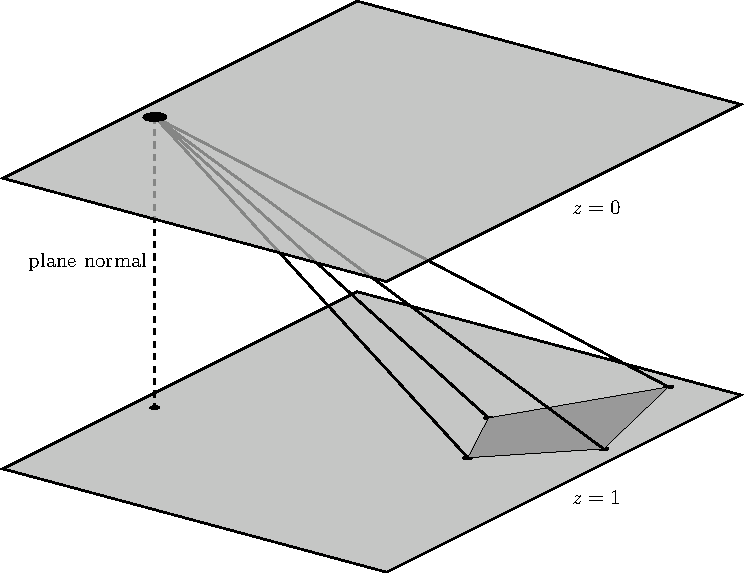
\includegraphics[width=\linewidth]{../lecture_notes/images/prob_geom1.pdf}
    \end{column}
\end{columns}
\end{frame}

\begin{frame}[t]{The importance of parameterization -- Example 2}
\begin{columns}
    \begin{column}{0.5\textwidth}
        \begin{minipage}[t][\textheight][t]{\textwidth}
        \theimportanceTwoHeight
        \begin{itemize}
        \item The mobile platform rotates about the
        plane normal (or $z$-axis) by an angle $\phi$.
        \item Translation parallel to the ground plane~$\mat{t}=(t_x,\,t_y,\,0)^{\T}$.
        \item Induced homography
        \begin{equation*}\label{eq:Hplanar}
            \mat{H} \sim \mat{R}_{\psi\theta}\mat{R}_{\phi}\mat{T}_{\mat{t}}\mat{R}_{\psi\theta}^{\T},
        \end{equation*}
        where $\mat{T}_{\mat{t}}=\mat{I}-\mat{tn}^{\T}$ and
        $\mat{n}=(0,\,0,\,1)^{\T}$ is a floor normal.
        \item The homography matrix can be made unique, \eg{} by imposing $\det{\mat{H}}=1$.
        \end{itemize}
        \end{minipage}
    \end{column}%
    \begin{column}{0.5\textwidth}
        \centering
        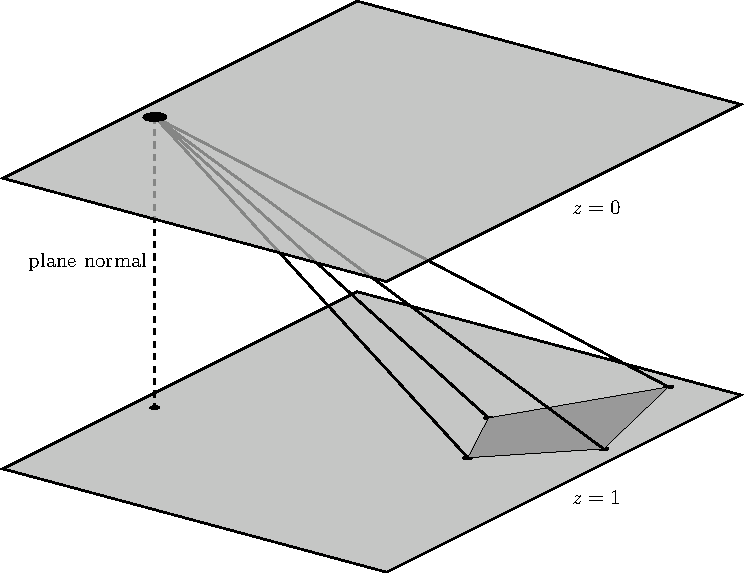
\includegraphics[width=\linewidth]{../lecture_notes/images/prob_geom1.pdf}
    \end{column}
\end{columns}
\end{frame}

\begin{frame}[t]{The importance of parameterization -- Example 2}
\begin{columns}
    \begin{column}{0.5\textwidth}
        \begin{minipage}[t][\textheight][t]{\textwidth}
        \theimportanceTwoHeight
        There are five degrees of freedom
        \begin{itemize}
            \item The fixed angles $\psi$ and $\theta$,
            \item The non-fixed angle $\phi$ and the translation components $t_x$ and $t_y$.
        \end{itemize}

        Minimal solver uses 2.5 point correspondences.
        \end{minipage}
    \end{column}%
    \begin{column}{0.5\textwidth}
        \centering
        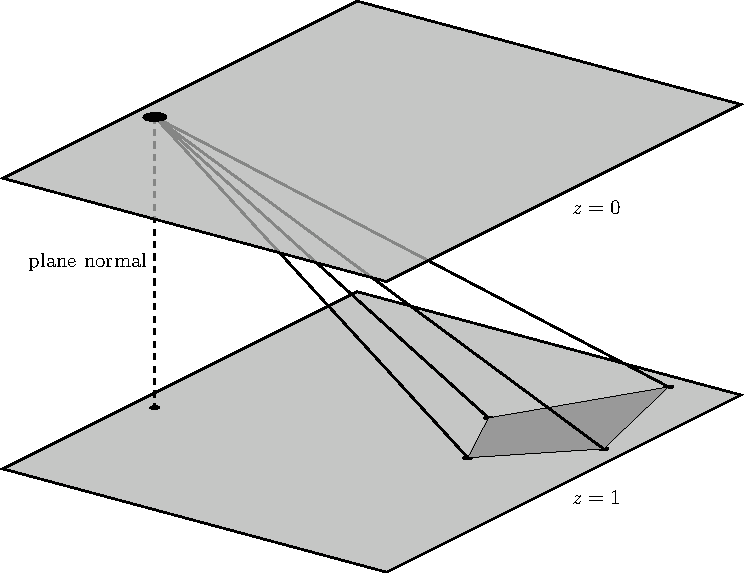
\includegraphics[width=\linewidth]{../lecture_notes/images/prob_geom1.pdf}
    \end{column}
\end{columns}
\end{frame}

\begin{frame}[t]{The importance of parameterization -- Example 2}
\begin{columns}
    \begin{column}{0.5\textwidth}
        \begin{minipage}[t][\textheight][t]{\textwidth}
        \theimportanceTwoHeight
        \textbf{Solver 1: Naive approach}

        Parameterize the rotation matrices
        \begin{equation*}
            \mat{R}_z(\phi) = \begin{bmatrix}
                \cos{\phi} & \sin{\phi} & 0 \\
                -\sin{\phi} & \cos{\phi} & 0 \\
                0 &0 &1
            \end{bmatrix}
        \end{equation*}
        where~$\cos^2{\phi}+\sin^2{\phi} = 1$, etc. Then use
        \[
            \mat{H} = \mat{R}_{\psi\theta}\mat{R}_{\phi}\mat{T}_{\mat{t}}\mat{R}_{\psi\theta}^{\T}\;.
        \]
        \end{minipage}
    \end{column}%
    \begin{column}{0.5\textwidth}
        \centering
        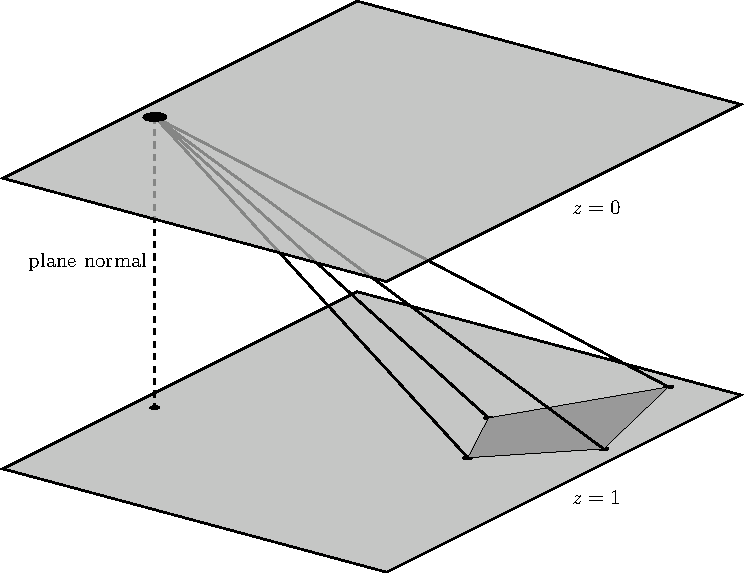
\includegraphics[width=\linewidth]{../lecture_notes/images/prob_geom1.pdf}
    \end{column}
\end{columns}
\end{frame}

\begin{frame}[t]{The importance of parameterization -- Example 2}
\begin{columns}
    \begin{column}{0.5\textwidth}
        \begin{minipage}[t][\textheight][t]{\textwidth}
        \theimportanceTwoHeight
        \textbf{Solver 1: Naive approach}

        The equations are:
        \[
        \begin{aligned}
            \mat{x}_1'\times \mat{Hx}_1 &= 0, &\quad \text{{\tiny (keep\,2\,eqs.)}} \\
            \mat{x}_2'\times \mat{Hx}_2 &= 0, &\quad \text{{\tiny (keep\,2\,eqs.)}} \\
            \mat{x}_3'\times \mat{Hx}_3 &= 0, &\quad \text{{\tiny (keep\,1\,eq.)}}
        \end{aligned}
        \]
        where
        $\mat{H} = \mat{R}_{\psi\theta}\mat{R}_{\phi}\mat{T}_{\mat{t}}\mat{R}_{\psi\theta}^{\T}$
        and
        \[
        \begin{aligned}
            \cos^2{\theta} + \sin^2{\theta} &= 0, \\
            \cos^2{\psi} + \sin^2{\psi} &= 0, \\
            \cos^2{\phi} + \sin^2{\phi} &= 0\;.
        \end{aligned}
        \]
        \end{minipage}
    \end{column}%
    \begin{column}{0.5\textwidth}
        \centering
        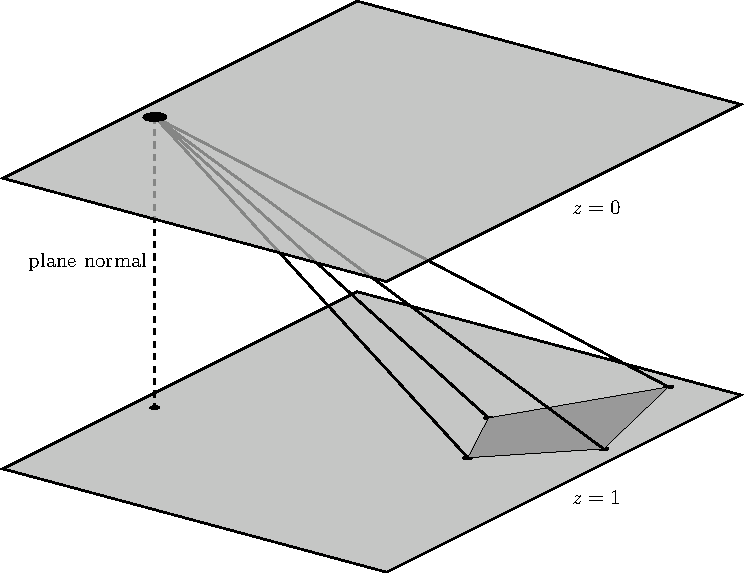
\includegraphics[width=\linewidth]{../lecture_notes/images/prob_geom1.pdf}
    \end{column}%
\end{columns}
\end{frame}

\begin{frame}[t]{The importance of parameterization -- Example 2}
\begin{columns}
    \begin{column}{0.5\textwidth}
        \begin{minipage}[t][\textheight][t]{\textwidth}
        \theimportanceTwoHeight
        \textbf{Solver 2: Re-parameterization}

        \begin{itemize}
            \item Align the overhead tilt!
            \item Camera matrices
            \[
                \begin{aligned}
                    \mat{P}_A &= [\mat{I}\,|\,\mat{0}], \\
                    \mat{P}_B &= [\mat{R}_{\mat{n}}(\phi)\,|\,-\mat{t}]
                \end{aligned}
            \]
            \item Induced homography
            \begin{equation*}\label{paper03:eq:h}
                \mat{H}= \mat{R}_{\mat{n}}(\phi)+\mat{t}\mat{n}^{ \T}\;.
            \end{equation*}
        \end{itemize}
        \end{minipage}
    \end{column}%
    \begin{column}{0.5\textwidth}
        \centering
        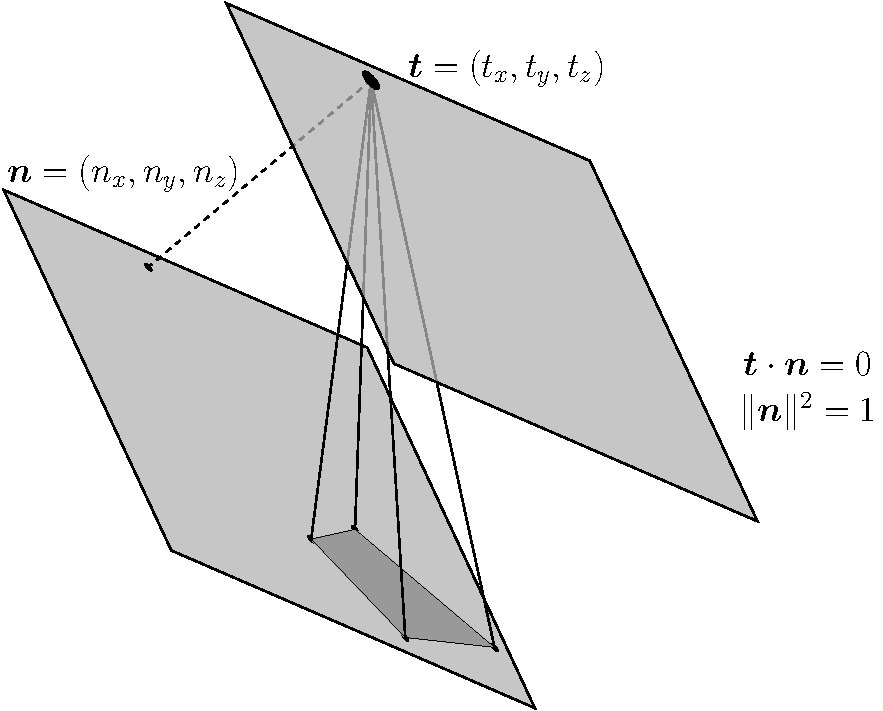
\includegraphics[width=\linewidth]{../lecture_notes/images/prob_geom1b.pdf}
    \end{column}
\end{columns}
\end{frame}

\begin{frame}[t]{The importance of parameterization -- Example 2}
\begin{columns}
    \begin{column}{0.5\textwidth}
        \begin{minipage}[t][\textheight][t]{\textwidth}
        \theimportanceTwoHeight
        \textbf{Solver 2: Re-parameterization}

        \begin{itemize}
            \item We have replaced several multiplications with addition $\longrightarrow$ lower degree polynomials
            \item No need to introduce auxilliary variables---just use quaternion representation.
            \item A single new constraint introduces, $\mat{t}\cdot\mat{n} = 0$.
        \end{itemize}
        \end{minipage}
    \end{column}%
    \begin{column}{0.5\textwidth}
        \centering
        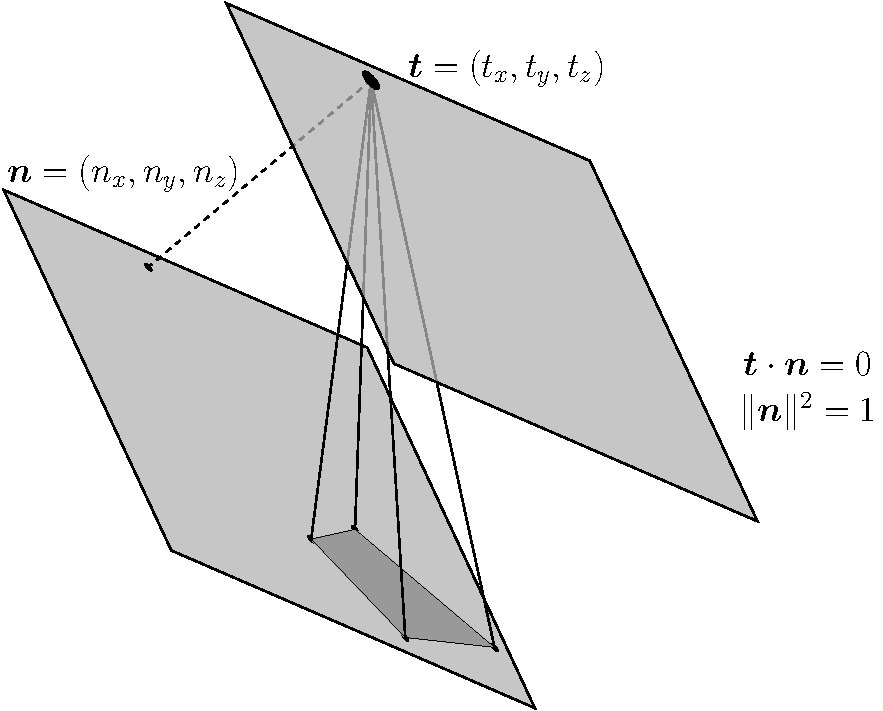
\includegraphics[width=\linewidth]{../lecture_notes/images/prob_geom1b.pdf}
    \end{column}
\end{columns}
\timetocode{}%
\end{frame}

\begin{frame}{The hidden variable trick}
The \emph{hidden variable trick} can be used when the equations are linear in one or more variables.
\begin{itemize}
    \item Reduces the number of unknowns, which potentially yields a smaller elimination template.
\end{itemize}
\end{frame}

\begin{frame}{The hidden variable trick -- Example 1}
Consider the following system
\begin{equation*}
\begin{aligned}
m_{11}xz + m_{12}x + m_{13}yz + m_{14}y + m_{15}z^2 + m_{16}z + m_{17} &= 0, \\
m_{22}xz + m_{22}x + m_{23}yz + m_{24}y + m_{25}z^2 + m_{26}z + m_{27} &= 0, \\
m_{32}xz + m_{32}x + m_{33}yz + m_{34}y + m_{35}z^2 + m_{36}z + m_{37} &= 0, \\
\end{aligned}
\end{equation*}
where~$m_{ij}\in\C$ are generic coefficients, and $x$, $y$ and $z$ are unknowns.
\end{frame}


\begin{frame}{The hidden variable trick -- Example 1}

The action matrix method is directly applicable, but
the system is linear in $x$ and $y$, hence we may write it as
\begin{equation*}\label{eq:specialnullvector}
\mat{M}(z)
\begin{bmatrix}
x \\
y \\
1
\end{bmatrix}
= 0,
\end{equation*}
where
\begin{equation*}
\mat{M}(z)=
\begin{bmatrix}
    m_{11}z + m_{12} & m_{13}z + m_{14} & m_{15}z^2 + m_{16}z + m_{17} \\
    m_{22}z + m_{22} & m_{23}z + m_{24} & m_{25}z^2 + m_{26}z + m_{27} \\
    m_{32}z + m_{32} & m_{33}z + m_{34} & m_{35}z^2 + m_{36}z + m_{37}
\end{bmatrix}\;.
\end{equation*}
\timetocode{}
\end{frame}

\begin{frame}{The hidden variable trick -- Example 1}
\begin{itemize}
\item We seek the one-dimensional nullspace of~$\mat{M}(z)$.
\item $\mat{M}(z)$ is rank deficient $\Rightarrow$ $\det(\mat{M}(z))=0$.
\item We get a quartic polynomial in~$z$
\begin{equation*}
    \det(\mat{M}(z)) =
    \alpha_4 z^4 +
    \alpha_3 z^3 +
    \alpha_2 z^2 +
    \alpha_1 z +
    \alpha_0 = 0,
\end{equation*}
where $\alpha_i\in\C$ only depend on~$m_{ij}$.
\item Closed-form solution available! No action matrix method necessary.
\item The remaining parameters can be obtained using SVD.
\end{itemize}
\timetocode{}
\end{frame}

\def\hiddenvariableTwoeHeight{\vspace{4mm}}
\begin{frame}[t]{The hidden variable trick -- Example 2}
\begin{columns}
    \begin{column}{0.5\textwidth}
        \begin{minipage}[t][\textheight][t]{\textwidth}
        \hiddenvariableTwoeHeight
        The scene plane $\pi$ and a camera's image plane $\pi'$ are related point-wise by the
        homography~$P$, so that $\alpha_i\mat{x}'_i=\mat{PX}_i$, where $\alpha_i$ is a scalar,
        $\mat{X}_i\in\pi$ and $\mat{x}'\in\pi'$. Let $\mat{X}_i$ and~$\mat{X}'_i$ be two points on the
        scene plane $\pi$ such that $\mat{X}'_i -\mat{X}_i=\mat{t}$. Then
        \begin{equation*}
            \alpha_i\mat{x}_i' = \mat{PX}'_i = \mat{PTX}_i = \mat{PTP}^{-1}\mat{x}_i=\mat{H_ux}_i,
        \end{equation*}
        where the homography $\mat{H_u}=\mat{PTP}^{-1}$ is called a conjugate translation.
        \end{minipage}
    \end{column}%
    \begin{column}{0.5\textwidth}
        \centering
        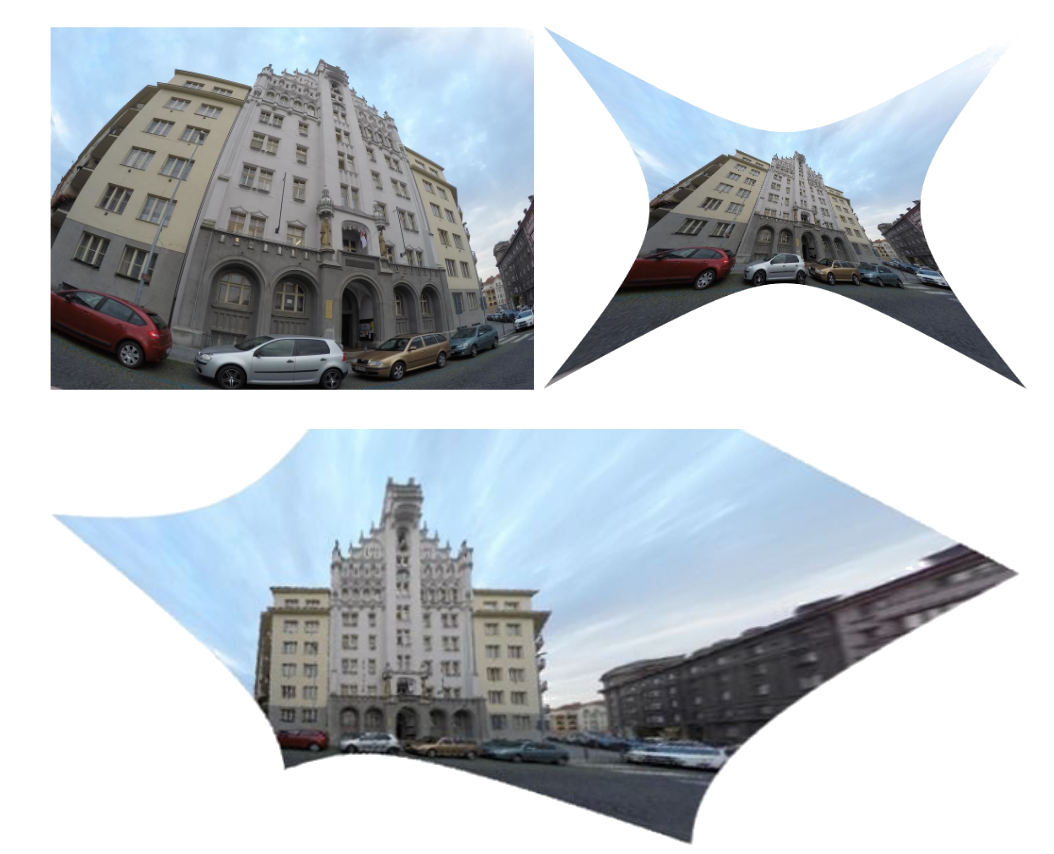
\includegraphics[width=\linewidth]{images/conjugate_trans.png}
        {\scriptsize Image credit: Pritts~\etal{} (2018).}
    \end{column}
\end{columns}
\end{frame}

\begin{frame}[t]{The hidden variable trick -- Example 2}
\begin{columns}
    \begin{column}{0.5\textwidth}
        \begin{minipage}[t][\textheight][t]{\textwidth}
        \hiddenvariableTwoeHeight
        We get
        \begin{equation*}
        \mat{H_u} \sim \mat{I}_3+s_i^{\mat{u}}\mat{ul}^\T,
        \end{equation*}
        where $\mat{I}_3$ is the $3\times 3$ identity matrix, and
        \begin{itemize}
        \item line $\mat{l}$ is the imaged scene plane’s vanishing line,
        \item point $\mat{u}$ is the vanishing direction of translation, which must meet the vanishing
              line~$\mat{l}$, \ie{} $\mat{l}^\T\mat{u} = 0$,
        \item and scalar $s_i^{\mat{u}}$ is the magnitude of translation in the direction $\mat{u}$ for
              the point correspondence $\mat{x}_i\leftrightarrow\mat{x}_i'$.
        \end{itemize}
        \end{minipage}
    \end{column}%
    \begin{column}{0.5\textwidth}
        \centering
        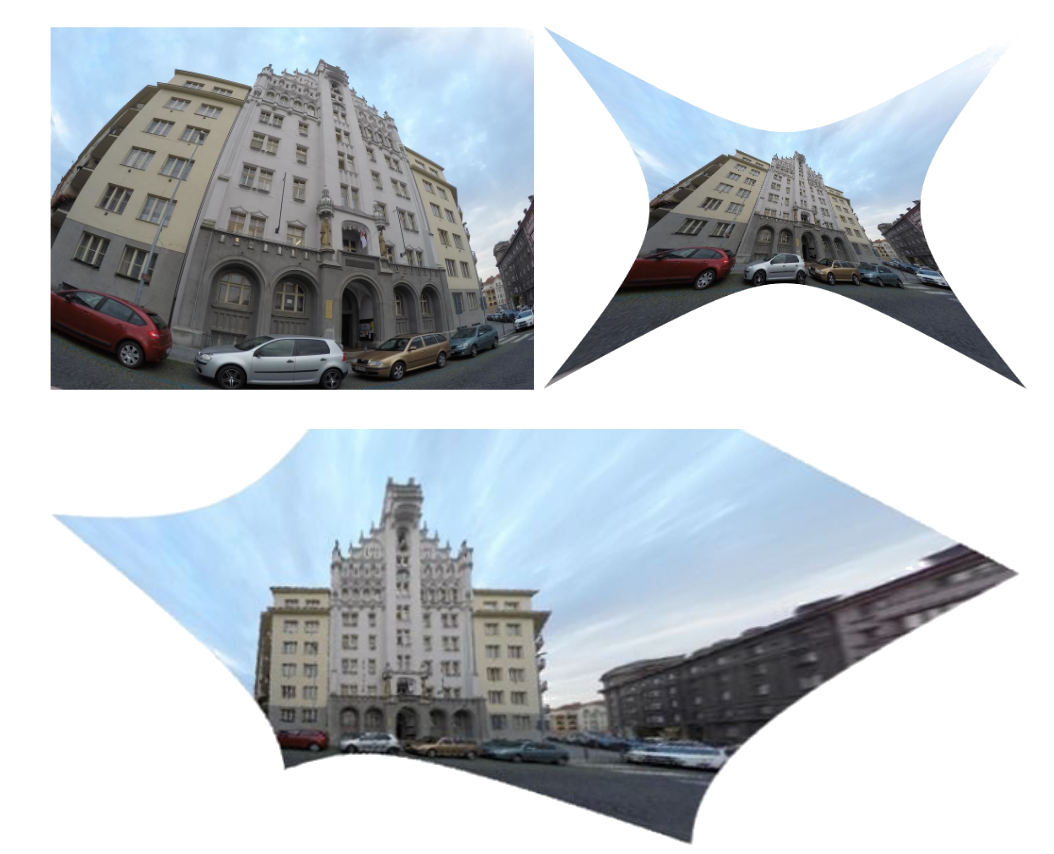
\includegraphics[width=\linewidth]{images/conjugate_trans.png}
        {\scriptsize Image credit: Pritts~\etal{} (2018).}
    \end{column}
\end{columns}
\end{frame}

\begin{frame}{Radial Distortion}
\begin{columns}
\begin{column}{0.6\textwidth}
        \begin{minipage}[t][\textheight][t]{\textwidth}
        \hiddenvariableTwoeHeight
        Fitzgibbon (2001): The division model
        \begin{equation*}
        \mat{x}_i^u = f(\mat{x}_i,\lambda)% = \begin{bmatrix}x_i\\y_i\\w_i\end{bmatrix}
        = \begin{bmatrix}x_i\\y_i\\1+\alert{\lambda}\,(x_i^2+y_i^2)\end{bmatrix}\;.
        \end{equation*}
        Benefits: a single distortion parameter~$\alert{\lambda}$ yields good results.
        \end{minipage}
\end{column}%
\begin{column}{0.4\textwidth}
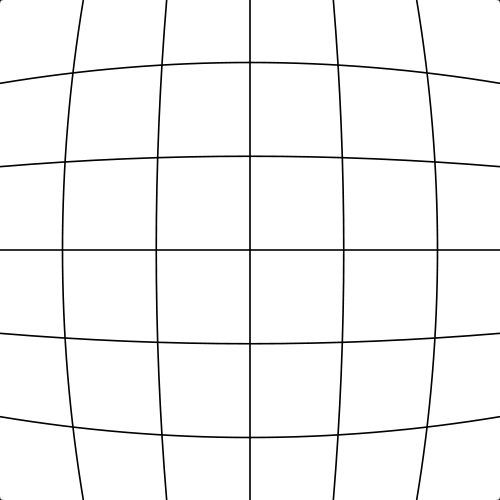
\includegraphics[width=0.9\linewidth]{images/distortion.png}
\end{column}%
\end{columns}%
\end{frame}

\begin{frame}[t]{The hidden variable trick -- Example 2}
\begin{columns}
    \begin{column}{0.5\textwidth}
        \begin{minipage}[t][\textheight][t]{\textwidth}
        \hiddenvariableTwoeHeight
        The problem:
        \begin{itemize}
            \item Add radial distortion,
            \item Fix scale: $l_3=1$ and $\norm{\mat{u}}=s_1^{\mat{u}}$.
            \item Let~$\bar{s}_i^{\mat{u}}\coloneqq s_i^{\mat{u}} / \norm{\mat{u}}$, then $\bar{s}_1^{\mat{u}}=1$.
            \item $\bar{s}_1^{\mat{u}} = \bar{s}_2^{\mat{u}} = 1$.
        \end{itemize}
We end up with
        \begin{itemize}
            \item 7 unknowns ($l_1$, $l_2$, $u_1$, $u_2$, $u_3$, $\bar{s}_3^{\mat{u}}$, $\lambda$),
            \item 7 equations---two equations
per point correspondences and the orthogonality constraint~$\mat{l}^\T\mat{u}= 0$.
        \end{itemize}
        Minimal solver: 3 points
        \end{minipage}
    \end{column}%
    \begin{column}{0.5\textwidth}
        \centering
        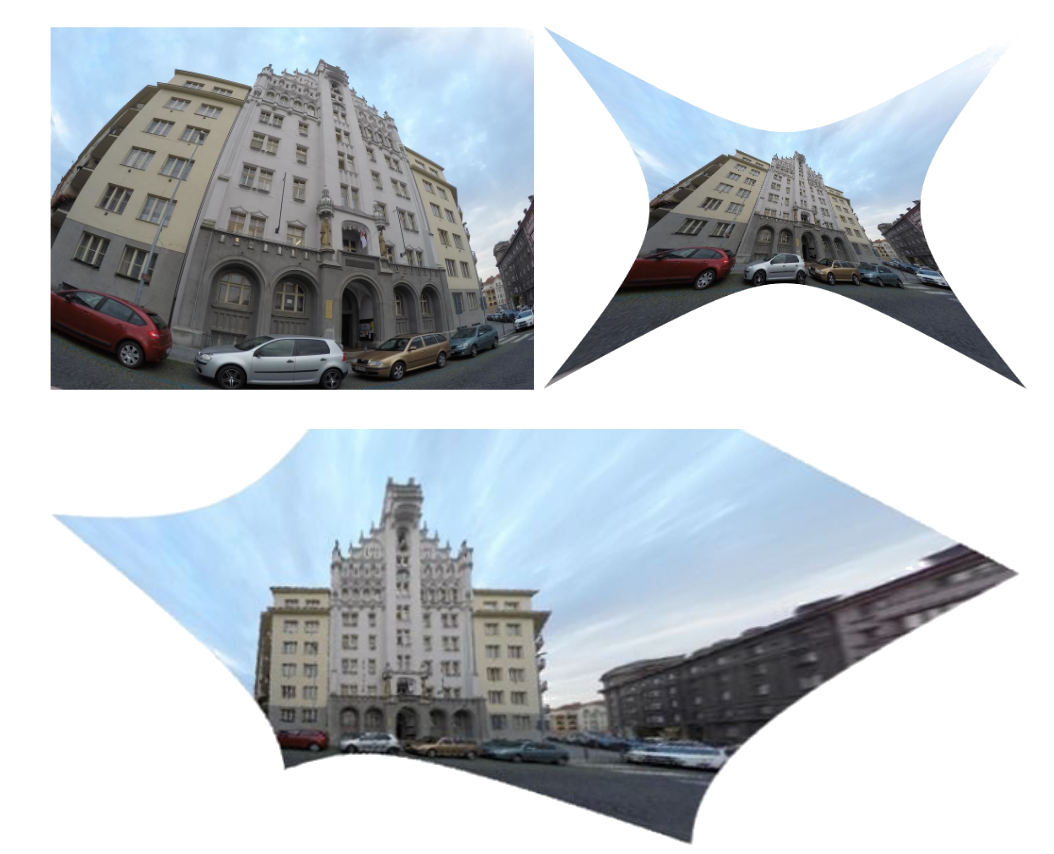
\includegraphics[width=\linewidth]{images/conjugate_trans.png}
        {\scriptsize Image credit: Pritts~\etal{} (2018).}
    \end{column}
\end{columns}
\end{frame}

\begin{frame}[t]{The hidden variable trick -- Example 2}
\begin{columns}
    \begin{column}{0.5\textwidth}
        \begin{minipage}[t][\textheight][t]{\textwidth}
        \hiddenvariableTwoeHeight
        Linear in~$\mat{u}$:
        \begin{equation*}
        \mat{M}(l_1,l_2,\bar{s}_3^{\mat{u}},\lambda)\begin{bmatrix} u_1 \\ u_2 \\ u_3 \\1\end{bmatrix} = 0
        \end{equation*}
        where $\mat{M} = \mat{M}(l_1,l_2,\bar{s}_3^{\mat{u}},\lambda)$ is a $7\times 4$ matrix.
        \end{minipage}
    \end{column}%
    \begin{column}{0.5\textwidth}
        \centering
        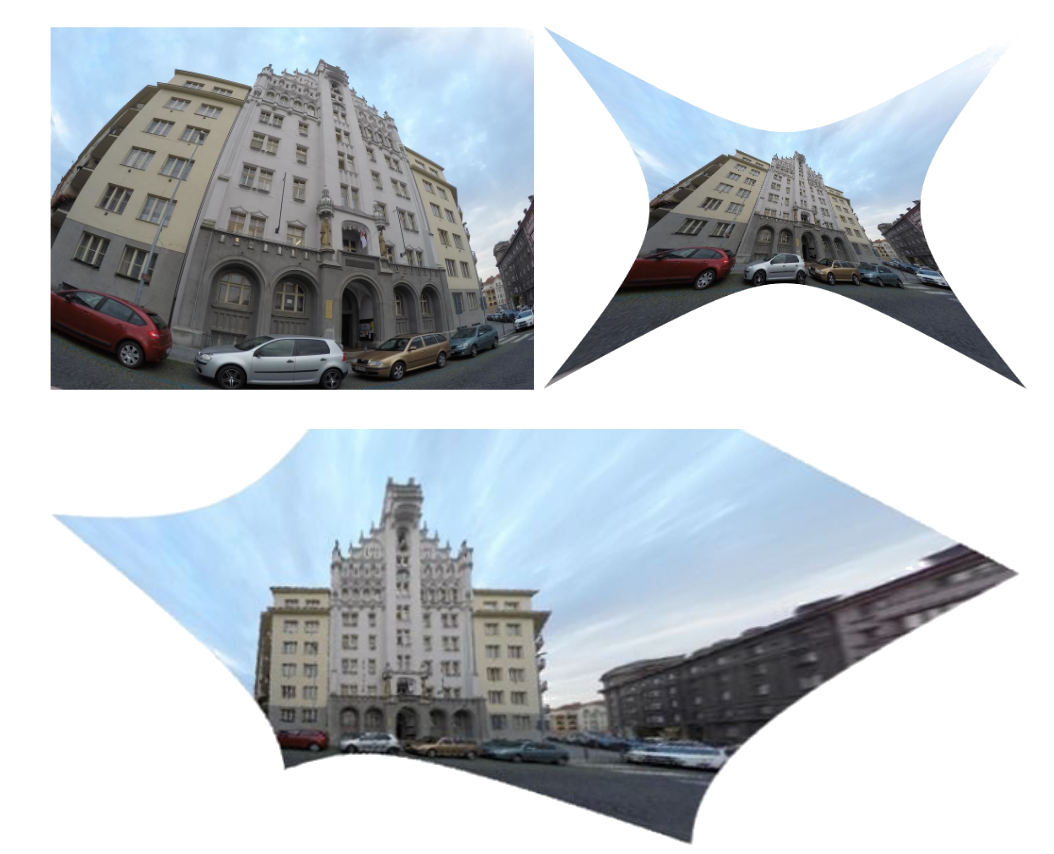
\includegraphics[width=\linewidth]{images/conjugate_trans.png}
        {\scriptsize Image credit: Pritts~\etal{} (2018).}
    \end{column}
\end{columns}
\end{frame}

\begin{frame}[t]{The hidden variable trick -- Example 2}
\begin{columns}
    \begin{column}{0.5\textwidth}
        \begin{minipage}[t][\textheight][t]{\textwidth}
        \hiddenvariableTwoeHeight
        It turns out that
        the matrix has a special structure, namely
        \begin{equation*}\label{eq:pritts-M}
        \mat{M} = \begin{bmatrix}
        m_{11} & m_{12} &      0 & m_{14} \\
        m_{21} & m_{22} &      0 & m_{24} \\
        m_{31} &      0 & m_{33} & m_{34} \\
        m_{41} &      0 & m_{43} & m_{44} \\
        m_{51} & m_{52} &      0 & m_{54} \\
        m_{61} &      0 & m_{63} & m_{64} \\
        l_1 & l_2 &   1 & 0
        \end{bmatrix}\;.
        \end{equation*}
        \end{minipage}
    \end{column}%
    \begin{column}{0.5\textwidth}
        \centering
        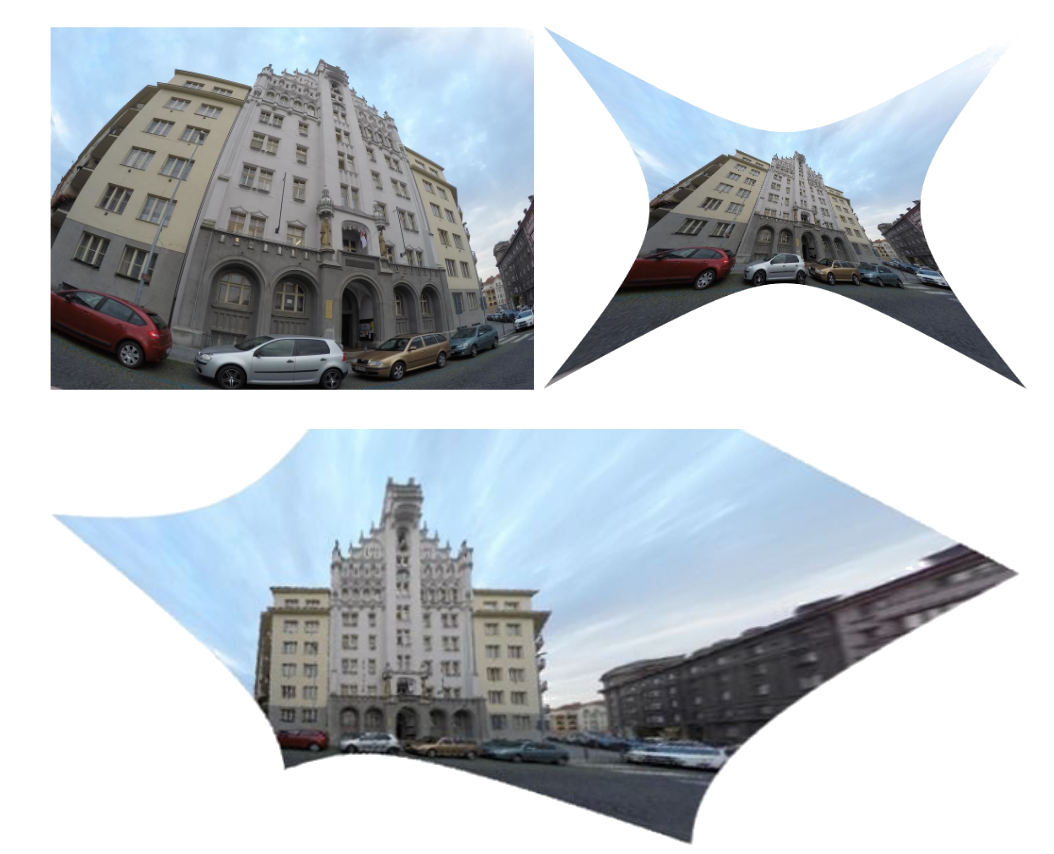
\includegraphics[width=\linewidth]{images/conjugate_trans.png}
        {\scriptsize Image credit: Pritts~\etal{} (2018).}
    \end{column}
\end{columns}
\timetocode{}
\end{frame}

\begin{frame}[t]{The hidden variable trick -- Example 2}
\begin{columns}
    \begin{column}{0.5\textwidth}
        \begin{minipage}[t][\textheight][t]{\textwidth}
        \hiddenvariableTwoeHeight
        The matrix $\mat{M}$ is rank deficient $\Rightarrow$
        all $4\times 4$ minors must vanish.

        There are $\binom{7}{4}=35$ minors. We have a problem with
        \begin{itemize}
            \item 4 unknowns
            \item 35 equations
        \end{itemize}

        We will return to this problem later.
        \end{minipage}
    \end{column}%
    \begin{column}{0.5\textwidth}
        \centering
        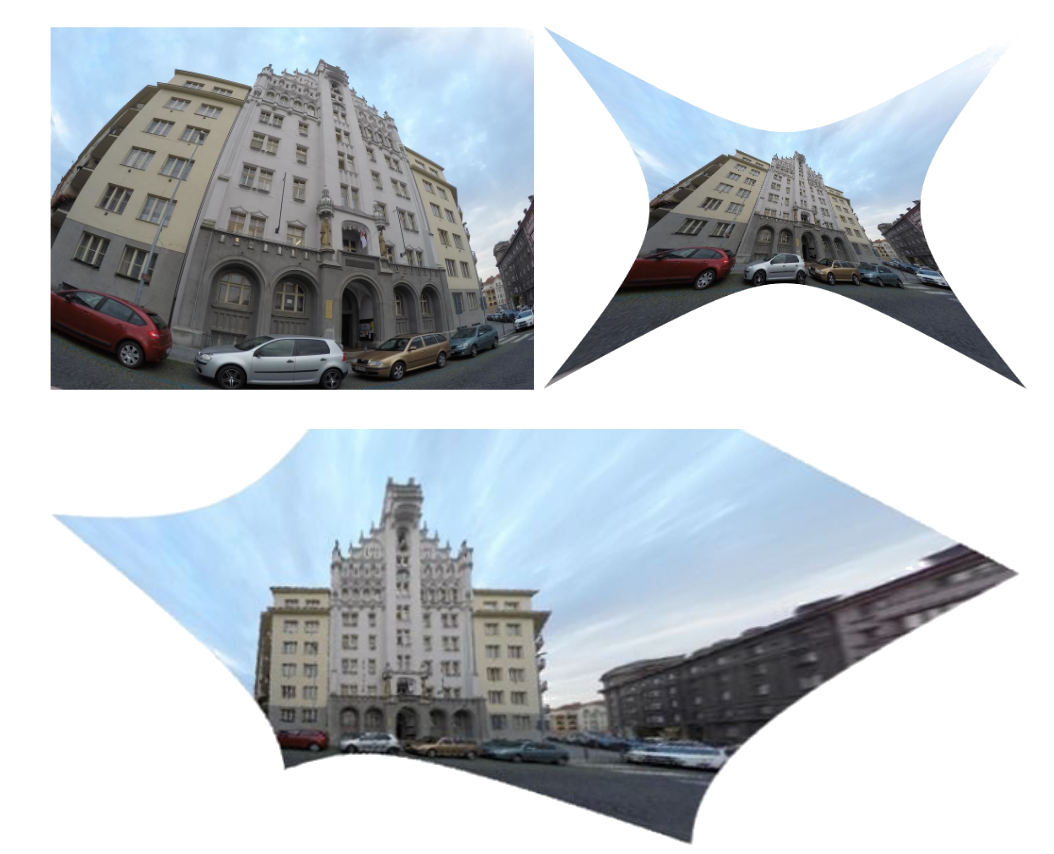
\includegraphics[width=\linewidth]{images/conjugate_trans.png}
        {\scriptsize Image credit: Pritts~\etal{} (2018).}
    \end{column}
\end{columns}
\end{frame}

\begin{frame}{Eliminating variables -- Example}
Sometimes we are able to eliminate variables even if there are no linear relationships. This
can be achieved using \emph{Gauss--Jordan elimination}.
\end{frame}

\begin{frame}{Eliminating variables -- Example}
Assume we have four unknowns $x$, $y$, $z$ and $w$, where $x^2+y^2=1$. We seek to solve
\begin{equation*}
    \mat{M}\mat{v} = 0,
\end{equation*}
where $\mat{M}\in\C^{3\times 9}$ is a coefficient matrix and the monomial vector is
\setcounter{MaxMatrixCols}{20}
\begin{equation*}
    \mat{v} = \begin{bmatrix}
            xw & x &
            yw & y &
            z^2 & zw^2 & z &
            w & 1
        \end{bmatrix}^\T\;.
\end{equation*}
\end{frame}

\begin{frame}{Eliminating variables -- Example}
Due to the constraint~$x^2+y^2=1$ we cannot use the hidden variable trick. But, we can still
eliminate $z$ by using Gauss--Jordan elimination. The corresponding system, after elimination, is
on the form
\begin{equation*}
\raisebox{-6pt}{ $\hat{\mat{M}} =$ }
\raisebox{-6pt}{\HUGE[}
\begingroup % keep the change local
\setlength\arraycolsep{2pt}
\begin{matrix}
%xw & x & yw & y & z^2 & zw^2 & zw & w & 1\\
z^2 & zw^2 & z & xw & x & yw & y & w & 1\\
    1 & & & \bullet & \bullet & \bullet & \bullet & \bullet & \bullet & \\
    & 1 & & \bullet & \bullet & \bullet & \bullet & \bullet & \bullet & \\
    & & 1 & \bullet & \bullet & \bullet & \bullet & \bullet & \bullet &
\end{matrix}
\endgroup
\raisebox{-6pt}{\HUGE]\;.}
\end{equation*}
\end{frame}

\begin{frame}{Eliminating variables -- Example}
We get
\begin{equation*}\label{paper04:eq:elim}
    \begin{aligned}
    z^2 + g_1(x,y,w)  &=  0,\\
    zw^2 + g_2(x,y,w)  &=  0,\\
    z + g_3(x,y,w)  &=  0,\\
    \end{aligned}
\end{equation*}
where~$g_i(x,y,w)$ are polynomials in the variables $x$, $y$ and~$w$.
Therefore
\begin{equation*}\label{paper04:eq:knowntilt1}
\begin{aligned}
    g_2(x,y,w) &= w^2 g_3(x,y,w), \\
    g_1(x,y,w) &= \left(g_3(x,y,w)\right)^2\;.
\end{aligned}
\end{equation*}
\end{frame}

\begin{frame}{Eliminating variables -- Example}
\textbf{Comparison:}

Before:
\begin{itemize}
    \item Four equations in four unknowns
    \item Max degree two
\end{itemize}

After:
\begin{itemize}
    \item Three equations in three unknowns
    \item Max degree four {\color{red}Note to self: Double check before workshop!}
\end{itemize}

\alert{Note:} Eliminating variables is often preferable, but there are cases when it is not.
Hard to say how it affects the overall performance\ldots You simply have to test yourself!
In such scenarios, it is nice to have an automatic generator for rapid prototyping.
\timetocode{}
\end{frame}

\begin{frame}{Saturation}
When is saturation useful?
\begin{itemize}
    \item To remove unwanted solutions!
        \begin{itemize}
            \item Physical (\eg{} focal length)
            \item Artificial (\eg{} introduced during parameterization)
        \end{itemize}
\end{itemize}
\end{frame}

\begin{frame}{The Rabinowitsch trick}
An alternative to saturation is the~\emph{Rabinowitsch trick}.
\vfill
\textbf{Comparison:} We want to exclude solutions~$f(\mat{x}) = 0$. Introduce auxiliary
variable~$x_0$, then

\emph{Rabinowitsh trick:} Add constraint~$x_0f(\mat{x})-1 = 0$

\emph{Saturation:} Add constraint $x_0-f(\mat{x}) = 0$ and saturate $x_0$.

\alert{Intuition:} Smaller elimination templates since the auxiliary variable $x_0$ is present
in a monomial with lower degree.
Furthermore, one may exclude the auxiliary variable~$x_0$ from the quotient ring basis
(when saturating polynomials).

\end{frame}

\begin{frame}{Saturation -- Example}
\begin{columns}
    \begin{column}{0.5\textwidth}
        \begin{minipage}[t][\textheight][t]{\textwidth}
        \hiddenvariableTwoeHeight
        Back to Pritts \etal{} (2018). Remember:
        \begin{equation*}\label{eq:pritts-M}
        \mat{M} = \begin{bmatrix}
        m_{11} & m_{12} &      0 & m_{14} \\
        m_{21} & m_{22} &      0 & m_{24} \\
        m_{31} &      0 & m_{33} & m_{34} \\
        m_{41} &      0 & m_{43} & m_{44} \\
        m_{51} & m_{52} &      0 & m_{54} \\
        m_{61} &      0 & m_{63} & m_{64} \\
        l_1 & l_2 &   1 & 0
        \end{bmatrix}\;.
        \end{equation*}
        $\mat{M}$ is rank deficient $\Rightarrow$
        all $4\times 4$ minors must vanish.
        Total: $\binom{7}{4}=35$ minors.

        \begin{center}
            \alert{Let's make a solver!}
        \end{center}
        \end{minipage}
    \end{column}%
    \begin{column}{0.5\textwidth}
        \centering
        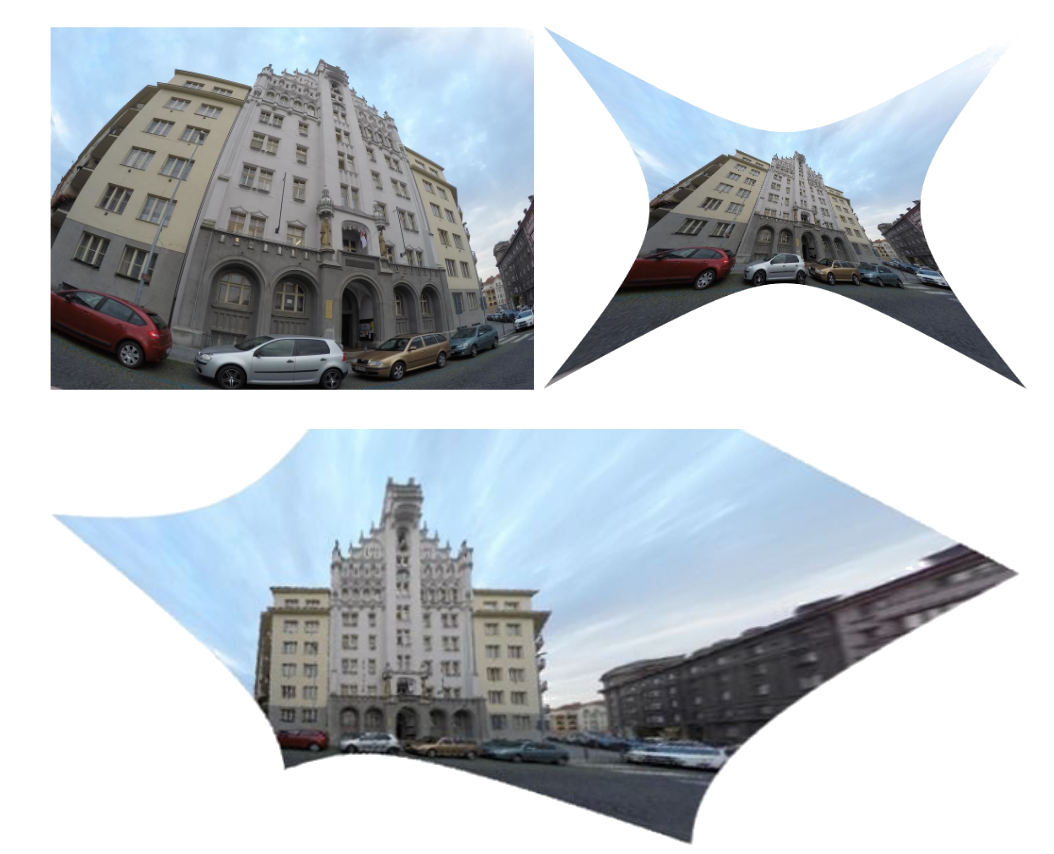
\includegraphics[width=\linewidth]{images/conjugate_trans.png}
        {\scriptsize Image credit: Pritts~\etal{} (2018).}
    \end{column}
\end{columns}
\timetocode{}
\end{frame}


\begin{frame}{Saturation -- Example}
We could not solve the previous problem. Macaulay2 cast an error
saying:
\begin{center}
    \texttt{module given is not finite over the base}
\end{center}

This means that there are infinitely many solutions. Why? Physically it seems unreasonable,
and if one goes back and creates a solver without using the hidden variable trick, we would
\emph{not} get this error.

\begin{itemize}
    \item[$\Rightarrow$] The hidden variable trick introduced a one-dimensional family of
                         spurious solutions!
\end{itemize}
\end{frame}

\begin{frame}{Saturation -- Example}
\textbf{Analysis:}

Where were these solutions introduced?
We used
\begin{equation*}
\mat{M}(l_1,l_2,\bar{s}_3^{\mat{u}},\lambda)\begin{bmatrix} u_1 \\ u_2 \\ u_3 \\1\end{bmatrix} = 0
\end{equation*}
where $\mat{M} = \mat{M}(l_1,l_2,\bar{s}_3^{\mat{u}},\lambda)$ is a $7\times 4$ matrix.

Then we created the 35 equations from the minors.

\end{frame}

\begin{frame}{Saturation -- Example}
\textbf{Analysis:}

The minors do not care about the structure of the null space!
The one-dimensional family of spurious solutions corresponds to solutions
of the form
\begin{equation*}
\mat{M}(l_1,l_2,\bar{s}_3^{\mat{u}},\lambda)\begin{bmatrix} u_1 \\ u_2 \\ u_3 \\\alert{0} \end{bmatrix} = 0
\end{equation*}
which are unwanted.
\end{frame}

\begin{frame}{Saturation -- Example}
\textbf{Solution:}

Use saturation! The unwanted solutions can be excluded by saturating any $3\times 3$ minor
from the first three columns\ldots

\begin{equation*}
\vcenter{\hbox{
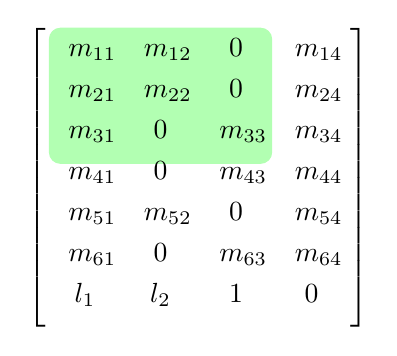
\begin{tikzpicture}[ampersand replacement=\&]
    \matrix[
        matrix of math nodes,
        row sep=0.65ex,
        column sep=2ex,
        left delimiter={[},right delimiter={]},
        nodes={text width=1.2em, text height=0.75ex, text depth=.5ex, align=center}
        ] (m)
        {
            m_{11} \& m_{12} \&      0 \& m_{14} \\
            m_{21} \& m_{22} \&      0 \& m_{24} \\
            m_{31} \&      0 \& m_{33} \& m_{34} \\
            m_{41} \&      0 \& m_{43} \& m_{44} \\
            m_{51} \& m_{52} \&      0 \& m_{54} \\
            m_{61} \&      0 \& m_{63} \& m_{64} \\
               l_1 \&    l_2 \&      1 \& 0      \\
        };
        \begin{scope}[on background layer]
            \node[fit=(m-1-1)(m-3-3), draw=green!30, fill=green!30, rounded corners] {};
        \end{scope}
\end{tikzpicture}
}}
     \begin{bmatrix}
        u_1 \\ u_2 \\ u_3 \\ 1
    \end{bmatrix} = 0
\end{equation*}
\end{frame}

\begin{frame}{Saturation -- Example}
\textbf{Solution:}

Use saturation! The unwanted solutions can be excluded by saturating any $3\times 3$ minor
from the first three columns\ldots

\begin{equation*}
\vcenter{\hbox{
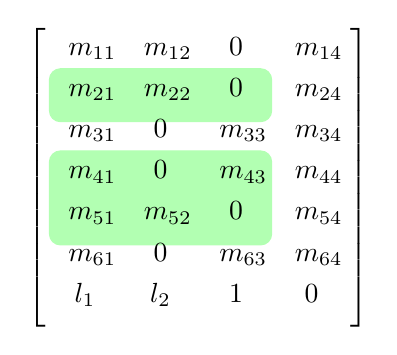
\begin{tikzpicture}[ampersand replacement=\&]
    \matrix[
        matrix of math nodes,
        row sep=0.65ex,
        column sep=2ex,
        left delimiter={[},right delimiter={]},
        nodes={text width=1.2em, text height=0.75ex, text depth=.5ex, align=center}
        ] (m)
        {
            m_{11} \& m_{12} \&      0 \& m_{14} \\
            m_{21} \& m_{22} \&      0 \& m_{24} \\
            m_{31} \&      0 \& m_{33} \& m_{34} \\
            m_{41} \&      0 \& m_{43} \& m_{44} \\
            m_{51} \& m_{52} \&      0 \& m_{54} \\
            m_{61} \&      0 \& m_{63} \& m_{64} \\
               l_1 \&    l_2 \&      1 \& 0      \\
        };
        \begin{scope}[on background layer]
            \node[fit=(m-2-1)(m-2-3), draw=green!30, fill=green!30, rounded corners] {};
            \node[fit=(m-4-1)(m-5-3), draw=green!30, fill=green!30, rounded corners] {};
        \end{scope}
\end{tikzpicture}
}}
     \begin{bmatrix}
        u_1 \\ u_2 \\ u_3 \\ 1
    \end{bmatrix} = 0
\end{equation*}
\end{frame}

\begin{frame}{Saturation -- Example}
\textbf{Solution:}

Use saturation! The unwanted solutions can be excluded by saturating any $3\times 3$ minor
from the first three columns\ldots \alert{but be smart!}

\begin{equation*}
\vcenter{\hbox{
    \tikzmark{pos}
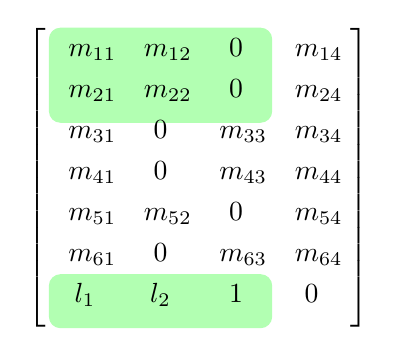
\begin{tikzpicture}[ampersand replacement=\&]
    \matrix[
        matrix of math nodes,
        row sep=0.65ex,
        column sep=2ex,
        left delimiter={[},right delimiter={]},
        nodes={text width=1.2em, text height=0.75ex, text depth=.5ex, align=center}
        ] (m)
        {
            m_{11} \& m_{12} \&      0 \& m_{14} \\
            m_{21} \& m_{22} \&      0 \& m_{24} \\
            m_{31} \&      0 \& m_{33} \& m_{34} \\
            m_{41} \&      0 \& m_{43} \& m_{44} \\
            m_{51} \& m_{52} \&      0 \& m_{54} \\
            m_{61} \&      0 \& m_{63} \& m_{64} \\
               l_1 \&    l_2 \&      1 \& 0      \\
        };
        \begin{scope}[on background layer]
            \node[fit=(m-1-1)(m-2-3), draw=green!30, fill=green!30, rounded corners] {};
            \node[fit=(m-7-1)(m-7-3), draw=green!30, fill=green!30, rounded corners] {};
        \end{scope}
\end{tikzpicture}
}}
     \begin{bmatrix}
        u_1 \\ u_2 \\ u_3 \\ 1
    \end{bmatrix} = 0
\end{equation*}

\begin{tikzpicture}[remember picture, overlay]
\draw[arrow]   ($ (pic cs:pos) +(-22mm,10mm) $) to [bend left,looseness=1.2] node[above] {Second order equation!} ($ (pic cs:pos) +(0mm, 36mm) $);
\end{tikzpicture}

\end{frame}

\begin{frame}{Saturation -- Example}
\textbf{Solution:}

Use saturation! The unwanted solutions can be excluded by saturating any $3\times 3$ minor
from the first three columns\ldots \alert{but be smart! Use the one with lowest degree}
\begin{equation*}
    f_{\text{sat}} =
        \begin{vmatrix}
        m_{11} & m_{12} & 0\\
        m_{21} & m_{22} & 0\\
        l_1 & l_2 &   1
        \end{vmatrix}
        =
        m_{11}m_{22}-m_{12}m_{21}\;.
\end{equation*}
Add an auxiliary variable $x_{\text{aux}}$ $\Rightarrow$ $x_{\text{aux}}-f_{\text{sat}}(l_1,l_2,\bar{s}_3^{\mat{u}},\lambda) = 0$, and saturate $x_{\text{aux}}$.
For comparison, we will also use the Rabinowitsch trick.
\timetocode{}
\end{frame}

\begin{frame}{A clever elimination strategy}
\textbf{Motivation:}
In computer vision, there are polynomial systems in which only the linear equations~$F_L$
depend on image measurements, while the nonlinear equations~$F_N$ stay the same, regardless of
image measurements.

Examples:
\begin{itemize}
\item Fundamental and essential matrix estimation,
\item Homographies given certain constraints on the motion,
and epipolar constraint generates linear equations that depend
\end{itemize}
\end{frame}

\begin{frame}{A clever elimination strategy}
\textbf{Offline:}
\begin{enumerate}
    \item Let $I = \langle F_N \rangle$ and consider the elimination
    ideal~$I_{X_L}=I\cap \C[X_L]$
    \item Compute the generators $G$ of $I_{X_L}$. These contain unknowns from $X_L$ only, \ie{}
    the unknowns appearing in the linear equations $F_L$.
\end{enumerate}
\end{frame}

\begin{frame}{A clever elimination strategy}
\textbf{Online:}
{\footnotesize
\begin{enumerate}
    \setcounter{enumi}{2}
    \item Rewrite the linear equations $F_L$ in the unknowns $X_L$ as $\mat{M}X_L= 0$, where $\mat{M}$
    is a coefficient matrix and the vector $X_L$ contains all unknowns from $X_L$.
    \item Compute a null space basis $\mat{N}$ of $\mat{M}$ and re-parametrize the unknowns $X_L=\mat{N}Y$. If the
    rank of $\mat{M}$ is $m_L$, \ie{} the equations in $F_L$ are linearly independent, $Y$ would contain
    $k=n_L - m_L$ new unknowns. Note that if all input equations in $F$ were homogeneous, we could
    set one of the unknowns in $Y$ to 1 (assuming it is non-zero) and then $k=n_L-m_L-1$.
    \item Substitute $X_L=NY$ into the generators $G$ of the elimination ideal $I_{X_L}$.
    \item Solve the new system of polynomial equations $G(Y) = 0$ (\eg{} using the Gröbner basis
    method and the precomputed elimination template for~\mbox{$G(Y) = 0$} obtained by using the automatic
    generator.
    \item Back-substitute to recover $X_L=\mat{N}Y$.
    \item Extend partial solutions for $X_L$ to solutions for $X$.
\end{enumerate}
}
\end{frame}

\begin{frame}{A clever elimination strategy -- Example 1}
\textbf{Example:} (Homework from Kalle) Estimating the essential matrix
\begin{center}
         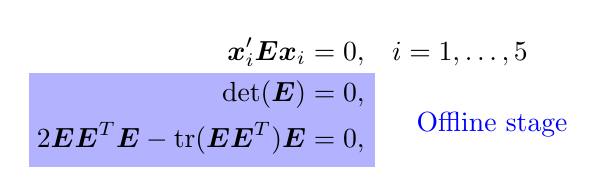
\begin{tikzpicture}
            \node[anchor=base,
                  path picture={\fill[blue!30] (-0.1,0.4)
                                rectangle (4.3,-0.9);}] (t1)
            {%
            $
            \begin{aligned}
                \mat{x}'_i\mat{E}\mat{x}_i &= 0, &i=1,\ldots,5\\
                \det(\mat{E}) &= 0,\\
                2\mat{EE}^\T\mat{E} - \tr(\mat{EE}^\T)\mat{E} &= 0,
            \end{aligned}
            $
            };
            \node[right of=t1, xshift=-5mm,yshift=-3.5mm] {\color{blue}Offline stage};
        \end{tikzpicture}
\end{center}

Only the input data $\mat{x}_i$ and $\mat{x}_i'$ change!

\alert{Note:} Online stage only! (Demazure proved the offline stage in 1988)
\end{frame}

\begin{frame}{A clever elimination strategy -- Example 1}
\textbf{Example:} (Homework from Kalle) Use five correspondences
\begin{equation*}
    \mat{M}\vectorize(\mat{E}) = 0,
\end{equation*}
where $\mat{M}$ is a $5\times 9$ coefficient matrix.
Express $\mat{E}$ in terms of the null space basis elements
\[
    \mat{E} = \sum_{i=1}^4\lambda_i\mat{E}_i,
\]
where we may fix the scale by letting~$\lambda_4=1$.
Insert this in the non-linear equations, \ie{} the rank and trace constraints.
\end{frame}


\begin{frame}[t]{A clever elimination strategy -- Example 2}
\begin{columns}
    \begin{column}{0.5\textwidth}
        \begin{minipage}[t][\textheight][t]{\textwidth}
        \theimportanceTwoHeight
        \textbf{Solver 3: Elimination strategy}

        Induced homography
        \begin{equation*}\label{paper03:eq:h}
            \mat{H}= \mat{R}_{\mat{n}}(\phi)+\mat{t}\mat{n}^{\T}
        \end{equation*}

        Let us do the offline stages! Denote the
        ideal~$I$ generated by
        \[
            \lambda \mat{H}-\mat{R}(\mat{q})-\mat{tn}^{T}=0,
        \]
        where~$\lambda$ is a scale factor and $\mat{t}\cdot\mat{n}=0$.
        We seek the elimination ideal~$I\cap\K[\mat{H}]$, for some suitable field~$\K$.

        \end{minipage}
    \end{column}%
    \begin{column}{0.5\textwidth}
        \centering
        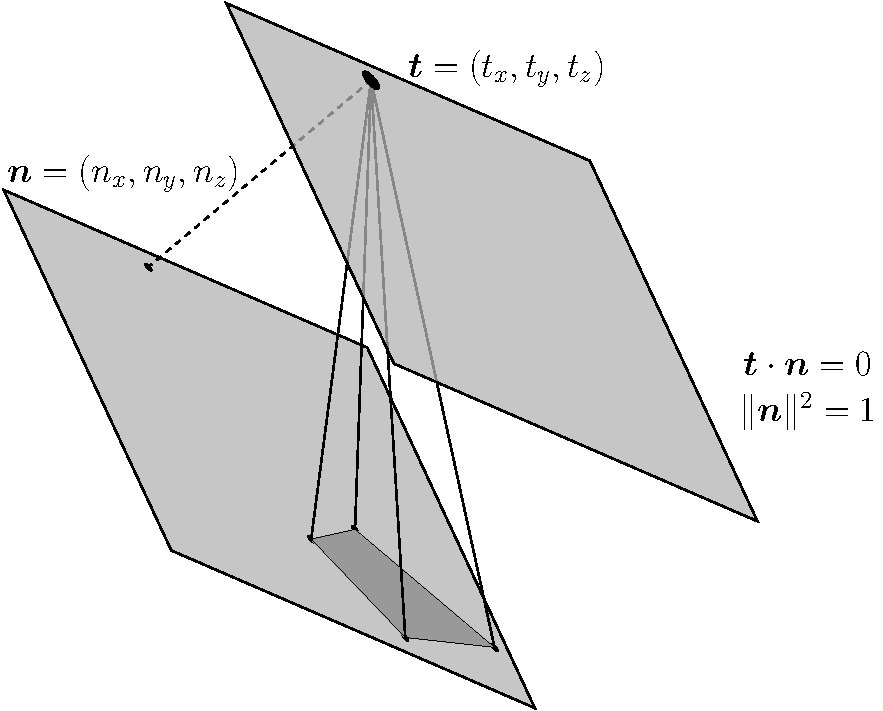
\includegraphics[width=\linewidth]{../lecture_notes/images/prob_geom1b.pdf}
    \end{column}
\end{columns}
\timetocode{}
\end{frame}

\begin{frame}[t]{A clever elimination strategy -- Example 2}
\begin{columns}
    \begin{column}{0.5\textwidth}
        \begin{minipage}[t][\textheight][t]{\textwidth}
        \theimportanceTwoHeight
        \textbf{Solver 3: Elimination strategy}

        We have the DLT equations
        \begin{equation*}
            \mat{x}_i'\times \mat{Hx}_i = 0, \quad i=1,\,2,\,3,
        \end{equation*}
        and choose two linearly independent rows (apart from the third pair). We get
        \begin{equation*}
            \mat{M}\vectorize(\mat{H}) = 0,
        \end{equation*}
        where $\mat{M}$ is a $5\times 9$ matrix.
        \end{minipage}
    \end{column}%
    \begin{column}{0.5\textwidth}
        \centering
        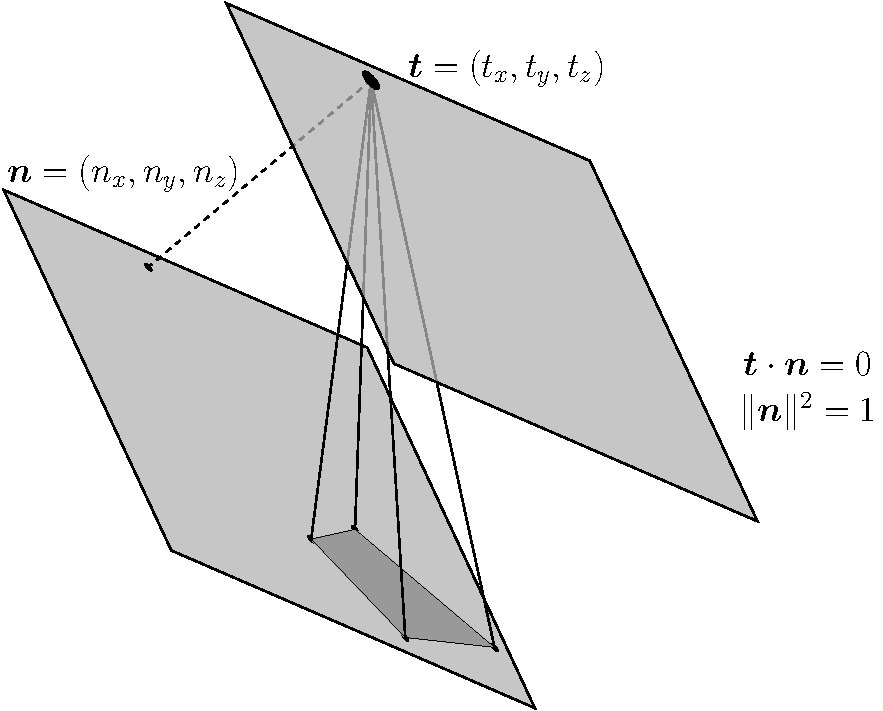
\includegraphics[width=\linewidth]{../lecture_notes/images/prob_geom1b.pdf}
    \end{column}
\end{columns}
\end{frame}

\begin{frame}[t]{A clever elimination strategy -- Example 2}
\begin{columns}
    \begin{column}{0.5\textwidth}
        \begin{minipage}[t][\textheight][t]{\textwidth}
        \theimportanceTwoHeight
        \textbf{Solver 3: Elimination strategy}

        Generally, $\nulldim(\mat{M})=4$, hence
        \begin{equation*}
            \mat{H} = \sum_{i=1}^4\lambda_i\mat{H}_i\;.
        \end{equation*}
        Insert into
        \begin{equation*}
        \begin{aligned}
            g_1(\lambda_1,\lambda_2,\lambda_3) &= 0, \\
            &\vdots \\
            g_{11}(\lambda_1,\lambda_2,\lambda_3) &= 0,
        \end{aligned}
        \end{equation*}
        \alert{Note: } Due to scale ambiguity, let $\lambda_4=1$.
        \end{minipage}
    \end{column}%
    \begin{column}{0.5\textwidth}
        \centering
        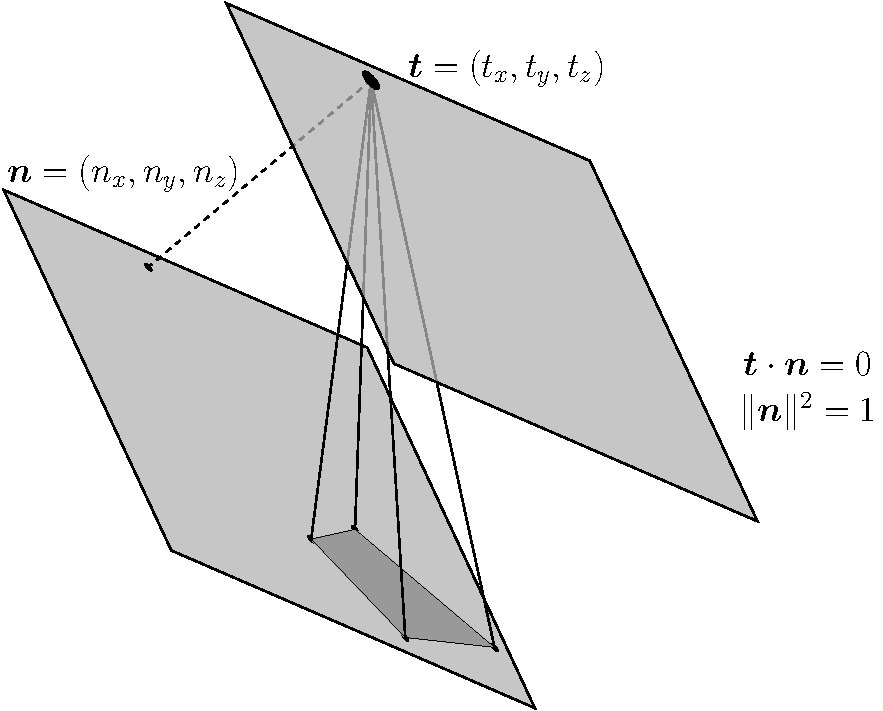
\includegraphics[width=\linewidth]{../lecture_notes/images/prob_geom1b.pdf}
    \end{column}
\end{columns}
\timetocode{}
\end{frame}

\begin{frame}{Further improvements}
Theory
\begin{itemize}
    \item Using $p$-fold symmetries,
    \item Beyond Gröbner bases,
    \item Polynomial Eigenvalue Problems (PEP),
    \item Resultant-based automatic generators,
    \item Large problems? Homotopy continuation.
\end{itemize}
Software
\begin{itemize}
    \item Generate in C++ and use fast solvers.
\end{itemize}
\end{frame}

\section{Time to make your own solver!}
\begin{frame}{Estimate the essential matrix}
Estimate the essential matrix from five point correspondences
\begin{center}
         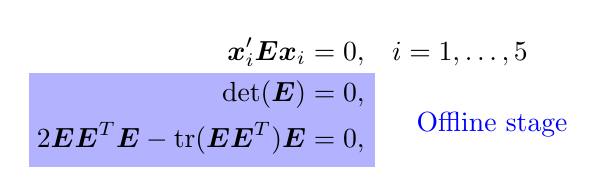
\begin{tikzpicture}
            \node[anchor=base,
                  path picture={\fill[blue!30] (-0.1,0.4)
                                rectangle (4.3,-0.9);}] (t1)
            {%
            $
            \begin{aligned}
                \mat{x}'_i\mat{E}\mat{x}_i &= 0, &i=1,\ldots,5\\
                \det(\mat{E}) &= 0,\\
                2\mat{EE}^\T\mat{E} - \tr(\mat{EE}^\T)\mat{E} &= 0,
            \end{aligned}
            $
            };
            \node[right of=t1, xshift=-5mm,yshift=-3.5mm] {\color{blue}Offline stage};
        \end{tikzpicture}
\end{center}
Express $\mat{E}$ in terms of the null space basis elements
\[
    \mat{E} = \sum_{i=1}^4\lambda_i\mat{E}_i,
\]
where we may fix the scale by letting~$\lambda_4=1$.
Insert this in the non-linear equations, \ie{} the rank and trace constraints.
\timetocode{}
\end{frame}

\section{Group exercise}

\begin{frame}{Group 1}
\textbf{Relative pose with one calibrated camera and one with unknown focal length}\\[8mm]
The fundamental matrix is~$\mat{E=FK}$, where $\mat{K}=\diag(f,\,f,\,1)$, and
\begin{equation*}
\begin{aligned}
    \mat{x}'_i\mat{F}\mat{x}_i &= 0, &i=1,\ldots,6\\
    \det(\mat{E}) &= 0, &\\
    2\mat{EE}^\T\mat{E}- \tr(\mat{EE}^\T)\mat{E} &= 0, &
\end{aligned}
\end{equation*}
\end{frame}

\begin{frame}{Group 2}
\textbf{Fundamental matrix with known rotation}\\[8mm]
For more info, see Example 8 and Example 11 from the lecture notes.
\end{frame}


\section{Suggestions for your individual project}

\begin{frame}{Problem 1}
\begin{columns}
    \begin{column}{0.5\textwidth}
        \textbf{Three (calibrated) cameras on a line}\\[8mm]
        \begin{itemize}
            \item How to parameterize?
            \item Which are the minimal cases?
        \end{itemize}
    \vspace{8mm}
    \footnotesize{(You may choose how many degrees of freedom you have in the rotation)}
    \end{column}%
    \begin{column}{0.5\textwidth}
        \centering
        \includestandalone[width=\linewidth]{tikz/3view_line}
    \end{column}
\end{columns}
\end{frame}

\begin{frame}{Problem 2}
\textbf{Panoramic stitching with a smartphone}\\[2mm]
Assume only rotation $\longrightarrow$ a homography~$\mat{H}$. Smartphones have an
IMU, hence a common reference direction exists. Then
\begin{equation*}
    \mat{H} = \mat{K}_2\mat{R}_2^\T\mat{R}_y\mat{R}_1\mat{K}_1^{-1},
\end{equation*}
where $\mat{R}_1$ and $\mat{R}_2$ is obtained from the IMU data. $\mat{R}_y$ is
a rotaiton about the $y$-axis.
Decide which case you want to look at
\begin{itemize}
    \item Focal length is unknown but the same,
    \item Focal length is unknown and possibly varying,
    \item Focal length and radial distortion parameter are unknown but the same,
    \item Focal length and radial distortion parameter are unknown and possibly varying.
\end{itemize}
\end{frame}

\end{document}
